 %
\documentclass[11pt]{article}

\usepackage[utf8]{inputenc}
\usepackage{amsmath}
\usepackage{amsthm}
\usepackage{amssymb}
\usepackage{mathabx} 
\usepackage{graphicx}
\usepackage{color} 
\usepackage{setspace} 
\usepackage{rotating}
\usepackage{natbib}
\usepackage{multirow}
\usepackage{xspace}
\usepackage{lscape}
%\usepackage{cite}
\usepackage{xr}
\usepackage{bbm}
\usepackage[normalem]{ulem}
\usepackage{newtxtext}
\usepackage{listings}
\usepackage{amssymb}
\usepackage[linesnumbered,lined,boxed,commentsnumbered,noend,ruled,vlined]{algorithm2e}

\usepackage{datetime}
\newdateformat{monthyeardate}{%
  \monthname[\THEMONTH], \THEYEAR}


\usepackage[labelfont=bf,labelsep=period,justification=raggedright]{caption}

\usepackage{hyperref}
\urlstyle{rm}
\hypersetup{
  colorlinks,
  urlcolor=blue,
  linkcolor=black,
  citecolor=black
}

% Text layout
\oddsidemargin 0in
\evensidemargin 0in
\topmargin -.5in
\textwidth 6.5in
\textheight 9in


% Remove brackets from numbering in List of References
\makeatletter
\renewcommand{\@biblabel}[1]{\quad#1.}
\newcommand{\smallCom}[1]{\marginpar{\tiny{#1}}}
\newcommand{\vect}[1]{\boldsymbol{\mathbf{#1}}}
\newcommand{\ld}{\mathcal{L}}
\newcommand{\ignore}[1]{}
\newcommand{\mcref}{\textsc{McRef}\xspace}
\newcommand{\E}{\mathbb{E}}
\newcommand{\X}{\vect{X}}
\newcommand{\M}{\mathcal{M}}
\newcommand{\Tr}{\mathcal{T}}
\newcommand{\B}{\vect{B}}
\newcommand{\Y}{\vect{Y}}
\newcommand{\G}{\vect{G}}
\newcommand{\T}{\vect{\Theta}}
\newcommand{\I}{\mathbb{I}}
\newcommand{\Ip}{\mathcal{I}(p,l)}
\newcommand{\Ib}{\mathcal{I}(b,l)}
\newcommand{\GT}{\G\T}
\newcommand{\Mref}{\M_{ref}}
\newcommand{\Mhyp}{\M_{hyp}}
\newcommand{\Mnull}{\M_{null}}
\newcommand{\Pref}{\widetilde{P}}
\newcommand{\rbf}{\text{BF}}
%\newcommand{\hbf}{\text{BF}}
\newcommand{\Om}{\Omega}
\newcommand{\GTref}{\widetilde{\GT}}
\newcommand{\Gref}{\widetilde{\G}}
\newcommand{\Tref}{\widetilde{\T}}
\newcommand{\1}{\mathbbm{1}}
\newcommand{\Z}{\vect{Z}}
\newcommand{\Zref}{\widetilde{\Z}}
\newcommand{\Omref}{\widetilde{\Om}}
\newcommand{\Fext}{F_{Z}}
\newcommand{\troot}{\theta_{root}}
\newcommand{\Gc}{\G_c}
\newcommand{\Gm}{\G_m}
\newcommand{\gp}{G-PhoCS }
\def\comb{\rotatebox[origin=c]{90}{$\exists$}}
\newcommand{\Mcomb}{\M_{\comb}}
\newcommand{\Gcomb}{\G_{\comb}}
\newcommand{\Tcomb}{\T_{\comb}}
\newcommand{\pcomb}{\p_{\comb}}
\newcommand{\tmin}{\tau_{\text{min}}}
% Two lines from genres
\def\@cite#1#2{(#1\if@tempswa , #2\fi)}
\def\@biblabel#1{}

\newtheorem{claim}{Claim}
\newtheorem{lemma}{Lemma}
\newtheorem{corollary}{Corollary}
\newtheorem{definition}{Definition}


\newcommand{\eqdef}{\stackrel{\Delta}{=}}		
\DeclareMathOperator*{\argmin}{\arg\!\min}

\newcommand{\taus}{\vect\tau}
\newcommand{\thetas}{\vect\theta}
\newcommand{\migs}{\vect{m}}


\newcommand{\thref}{\widetilde{\thetas}}
\newcommand{\taref}{\widetilde{\taus}}
\newcommand{\migref}{\widetilde{\migs}}

\newcommand{\thcomb}{\theta_{comb}}
\newcommand{\tacomb}{\tau_{comb}}

\def\comb{\rotatebox[origin=c]{90}{$\exists$}}




% Default fixed font does not support bold face
\DeclareFixedFont{\ttb}{T1}{txtt}{bx}{n}{10} % for bold
\DeclareFixedFont{\ttm}{T1}{txtt}{m}{n}{10}  % for normal

% Custom colors
\usepackage{color}
\definecolor{deepblue}{rgb}{0,0,0.5}
\definecolor{deepred}{rgb}{0.6,0,0}
\definecolor{deepgreen}{rgb}{0,0.5,0}

\usepackage{listings}

% Python style for highlighting
\newcommand\pythonstyle{\lstset{
language=Python,
basicstyle=\ttm,
otherkeywords={self},             % Add keywords here
keywordstyle=\ttb\color{deepblue},
emph={recursive_num_coals,recursive_coal_stats},% Custom highlighting
emphstyle=\ttb\color{deepred},    % Custom highlighting style
stringstyle=\color{deepgreen},
frame=tb,                         % Any extra options here
showstringspaces=false            % 
}}


% Python environment
\lstnewenvironment{python}[1][]
{
\pythonstyle
\lstset{#1}
}
{}

% Python for external files
\newcommand\pythonexternal[2][]{{
\pythonstyle
\lstinputlisting[#1]{#2}}}

% Python for inline
\newcommand\pythoninline[1]{{\pythonstyle\lstinline!#1!}}

\newenvironment{tightcenter}{%
  \setlength\topsep{0pt}
  \setlength\parskip{0pt}
  \begin{center}
}{%
  \end{center}
}

\graphicspath{ {../images/} }

\author{Ron Visbord}
% \newcommand{\smallCom}[1]{\marginpar{\tiny{#1}}}

\begin{document}


\begin{titlepage}
	\centering
	
\includegraphics[width=0.4\textwidth]{IDC_logo}\par\vspace{2cm}
	{\huge The Interdiciplinary Center, Herzliya \par}
	{\Large Efi Arazi School of Computer Science \par}
	{\Large M.Sc. Program - Research Track \par}
	
	\vspace{1cm}
	
	\vspace{1.5cm}
	{\Huge A New Bayesian Method for Comparing Demographic Models \par}
	\vspace{3cm}
	{\large by\par}
	{\large\bfseries Ron Visbord\par}
	
	\vspace{2cm}
	{M.Sc. dissertation, submitted in partial fulfillment of the requirements\par}
	{for the M.Sc. degree, research track, School of Computer Science\par}
	{The Interdisciplinary Center, Herzliya}
	
	\vfill
	
	% Bottom of the page
	{\large \monthyeardate\today \par}
	
\end{titlepage}

\newpage

This work was carried out under the supervision of Dr. Ilan Gronau from the Efi Arazi School of Computer Science, The Interdiciplinary Center, Herzliya.

\newpage

\section*{Abstract}
High throughput sequencing has greatly improved our ability to investigate the evolutionary history of species using detailed demographic models. A popular approach for inferring parameters in these demographic models is by sampling genealogical histories at many short unlinked loci using a Markov Chain Monte Carlo algorithm. The use of explicit coalescent models by these methods makes them powerful for inferring demographic parameters, but they are limited in their ability to assess the fit of the inferred model to data. The purpose of this research is to examine a new approach, based on Relative Bayes Factors, for using genealogy samples to compare different evolutionary hypotheses. 


\newpage

\tableofcontents

\newpage



















%%%%%%%%%%%%%%%%%%%%%%%%%%%%%%%%%%%%%%%%%%%%%%%%%%%%%%%%%%%%%%%%%%%%%%%%%%%%%%%%%
%%%%%%%%%%%%%%%%%%%%%%%%%%%% HERE STARTETH THE PAPER %%%%%%%%%%%%%%%%%%%%%%%%%%%%
%%%%%%%%%%%%%%%%%%%%%%%%%%%%%%%%%%%%%%%%%%%%%%%%%%%%%%%%%%%%%%%%%%%%%%%%%%%%%%%%%



\section{Introduction}

In recent years, advances in high throughput DNA sequencing have made it easy to sequence many genomes of individuals from closely related species. This allows evolutionary biologists to examine the evolution of recently diverged species by employing data-intensive computational methods and statistical models.
%
Typically, an evolutionary biologist, having obtained and aligned genome sequences of individuals from relative species or populations, would like to reconstruct the evolutionary history of the sequenced individuals. This evolutionary history includes a series of population splits, population size changes and post-divergence gene flow.\\
%
The job of reconstructing this evolutionary history may be viewed as two seperate tasks; First, one must find the phylogenetic model structure $\M$. This is a tree-like graph which represents the ancestral relation between all relevant populations, as well as any migration bands between populations. This task is often referred to as \textbf{Model selection}. Second, having obtained the model structure, one must find the phylogenetic model parameters. These are the specific parameter values or distributions of the model, such as population divergence times, population sizes and migration rates. This is the task of \textbf{Parameter Inference}. [TODO - rephrase to focus on the components of the evolutionary history, not the reconstruction process]\\
%
One successful approach for parameter inference has been to assume the model structure $\M$, and to explicitly represent the genealogy of the sequenced individuals at short unlinked loci. These local genealogies are used along-side the target model parameters as hidden variables in a Markov chain Monte Carlo (MCMC) sampling algorithm, effectively integrating out the information on genealogical relationships between individuals and producing Bayesian estimates of the target parameters [TODO - shorten sentence] [TODO - reference said methods] .
%
These methods have two key advantages: 1) The full probabilistic generative model of the data at their core allows modeling more complex evolutionary history, with more free parameters; 2) The parameter values sampled by MCMC provide means to assess the uncertainty in the resulting estimates.
%
However, because these methods condition on a given model structure $\M$, they provide no straightfprward solution to the model selection problem.
%
In principle, measuring of model fit can be approximated by using importance sampling on the approximated posterior distribution, but standard methods for doing this are statistically inefficient [TODO - reference].
%
This leaves us with no robust method for comparing the fit of different structures pf evolutionary history to a given genomic data set.\\
%
\\
The goal of our research is thus to \textbf{utilize bayesian parameter inference methods to perform robust model selection}.
%
We accomplish this by introducing the concept of \textbf{Reference Models}, which are base-line phylogenetic structures used to asses model fit to data within a specific context, allowing us to choose between competing model candidates. [TODO - maybe borrow the phrasing "evaluate the fit of model M by estimating its likelihood relative to
the reference model". maybe also mention Relative Bayes Factors]
%
We will start by overviewing existing work in the field and laying down the background and common notations for phylogenetic models and parameter inference.
%
We will then formally develop from scratch the concept of reference models, how the relate to phylogenetic population models, how they are used as model comparison criteria, and why they are advantageous over existing methods for model selection. 
%
We will then explain in detail our implementation of reference-model-based model selection based on the \gp parameter-inference framework, nicknamed \textbf{McRef} due to it's employment of reference models in the MCMC process.
%
Finally we will share empirical results from our model-comparison experiments, showcasing the advantages and limitations of our implementation.

\subsection{Other Relevant Work}

Discuss structure+parameter inference methods here - 

\begin{itemize}
\item general methods (non bayesian) for history reconstruction. what are the drawbacks in "likelihood-based" approaches?

\item importance-sampling based

\item thermodynamic stuff for improving harmonic-mean (hopefully these methhods can also be applied on mcref)

\end{itemize}

\section{Preliminaries}
\subsection{Demographic models and Bayesian inference}




A probabilistic demographic model $\M$ uses a parameterized demographic history to define a probability distribution over observed genomic data $\X$.
%
The structural components of $\M$, which we assume are fixed, consist of a population phylogeny $\Tr$ and a collection
of migration bands $B$ that indicate ordered pairs of populations between which gene flow is allowed.
%
The free parameters of $\M$, denoted here by $\T$, consist of divergence times, $\taus=\{\tau_p:p \text{ is an ancestral population of } \Tr\}$,
effective population sizes, $\thetas=\{\theta_p: p \text{ is a population in } \Tr\}$, and migration rates, $\migs=\{m_b:b \in B\}$.
%
All model parameters are scaled by mutation rate.
%
The model $\M$ is thus defined by specifying the structural components $(\Tr,B)$ and a prior distribution over the free parameters of the model $P(\T|\M)$.
%
The conditional probability distribution for the observed genomic data, $P(\X|\M,\T)$, is defined by standard models for molecular evolution and population genetics (e.g., \cite{JUKECANT69,KING82A}) [TODO - fix references].
%
The objective of demography inference methods is to infer values for $\T$ that have high joint probability with the data:
$P(\X,\T|\M)=P(\T|\M)P(\X|\M,\T)$.

%
Because the conditional probability $P(\X|\M,\T)$ does not typically have a closed-form expression, an increasingly popular approach for
inference is to introduce additional hidden variables $\G$, which represent genealogical relationships
between the sampled individuals.
%
The benefit of this is that given the genealogical information, the data $\X$ becomes independent of the model $\M$ and parameters $\T$,
and the likelihood can be expressed as a product of three efficiently computable terms:
%
%
\begin{equation}\label{eq:likelihood}
 P(\X,\G,\T|\M) ~=~ P(\T|\M) P(\G|\M,\T) P(\X|\G)~.
\end{equation}
%
%

This joint probability function may be used by a Markov chain Monte Carlo (MCMC) algorithm to generate a sample of the model parameters
together with the genealogies according to a probability distribution approximating the posterior, $P(\G,\T|\M,\X)$.
%
Consequently, the sampled parameter values have high joint probability with the data.
%
A major advantage of this approach to inference is that it is extremely flexible and can be applied to a wide range of demographic models and
different types of genomic data.
%




\subsection{\gp}

\gp is one such Bayesian demography inference method. It considers a model for sequence data at short unlinked loci, in which case 
$\G$ contains the information on the local tree in each locus, and distinct loci are assumed to be independent (e.g., \cite{NIELWAKE01,RANNYANG03,GRONETAL11}) [TODO - fix references]. In each MCMC iteration \gp proposes a new instace of $\G, \T$ and decides if to accept the proposal based on the ratio between complete likelihoods of the current instance and proposed instance. Equation \ref{eq:likelihood} shows the likelihood calculation used by \gp
%
\begin{equation}\label{eq:likelihood}
 P(\X,\G,\T|\M) ~=~ P(\T|\M) P(\G|\M,\T) P(\X|\G) ~=~ P(\T|\M) \prod_l P(\G_l|\M,\T) P(\X_l|\G_l).
\end{equation}

Where $P(\T|\M)$ is the prior probability of model parameters to take current values, $P(\G_l|\M,\T)$ is the probability of local genealogy $G_l$ given the model parameters, calculated under the Kingman Coalescent model, with special regard to migration events, and $P(\X_l|\G_l)$ is the local dna data likelihood given genealogy $G_l$.


\begin{figure}[h]
\centering
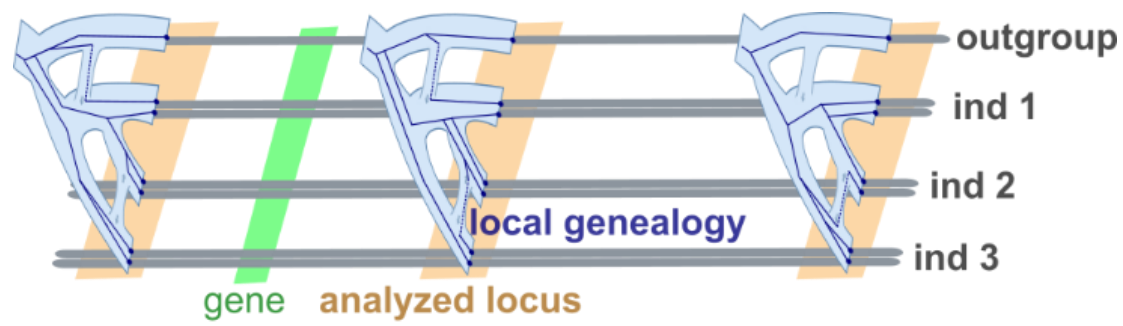
\includegraphics[width=0.8\textwidth]
{multiple_loci_across_sequence}
\captionsetup{width=.8\textwidth}
\caption{Given a small collection
of unphased genomes at tens of thousands of short unlinked neutrally evolving loci, and a population phylogeny model, \gp infers parameters $\T$ - population divergence times $\tau$ , ancestral population sizes $\theta$ and rates of post-divergence gene flow $m$. This is accomplished using MCMC sampling of local
genealogies jointly with model parameters according to an approximate posterior distribution for full Bayesian inference.}
\label{fig:multiple_loci_across_sequence}
\end{figure}


\subsection{The Model Comparison problem}
We introduce here an adaptation of demography inference methods such as \gp to the problem of model-selection, and more specifically model comparison. The Model Comparison Problem aims to \textbf{compare the fit of candidate structural models to sequence data}.
\begin{figure}[h]
\centering
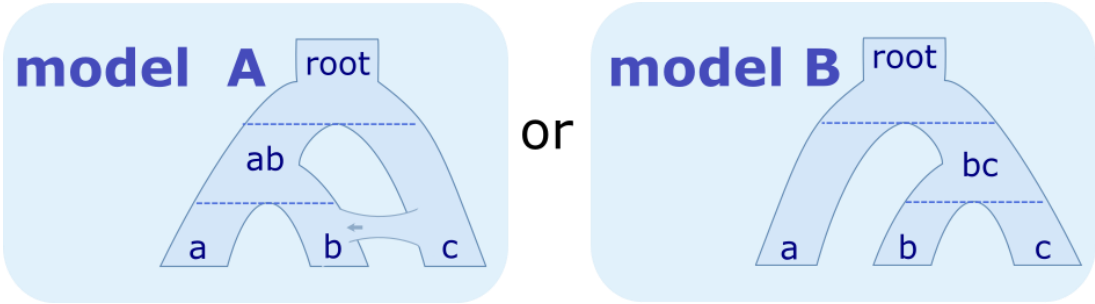
\includegraphics[width=0.8\textwidth]
{model_A__OR__model_b}
\captionsetup{width=.8\textwidth}
\caption{The model Comparison problem: \textit{“Given sequence data $X$ of samples from
relative populations, which of the candidate phylogenetic topologies $\M$ best fits the data?“}}
\label{fig:model_A__OR__model_b}
\end{figure}


The Model Comparison problem makes a distinction between structural components of model $\M$ ($\Tr$ and $B$) and parameter values $\T$. Model Comparison aims to compare different model structures.
%
In this study, building upon the \gp demography inference method and MCMC sampler, we develop the theoretical framework for a robust model-comparison scheme, and implement a method to compare multiple models and their fit to the data, this without analytically calculating $P(X|\M)$.
%
We bear in mind that in most cases researchers are interested only in qualitative claims about the structure
of the model and not in qualitative claims about specific parameter values. To keep our method as
general as possible, the comparison algorithm we present receives no parameters $\T$ and will thus
output a result pertaining only to the topology of the model. This will allow us to test \textit{structural
hypotheses} by integrating over parameter values.


\section{Methods}


\subsection{Estimating data likelihood via importance sampling}

A fundamental limitation of Bayesian demography inference methods is that they do not directly produce reliable measures of model fit.
%
Model fit is best captured by the marginal data likelihood, $P(\X|\M)$, whose computation involves integration over the space of unknown parameter values and genealogical relationships,
denoted jointly by $\GT$.
%
This high-dimensional integral may be approximated via importance sampling using a collection of instances $\{\GT^{(i)}\}$ sampled via MCMC conditioned on $\X$ and $\M$.
%
The approximation is established by expressing the inverse of the likelihood as an expected value under the posterior distribution of $\GT$ given $\M$ and $\X$:
%
%
\begin{small}
\begin{align}
%\frac{1}{\hbf(\M|\X)} ~~~ \triangleq~~
\frac{1}{P(\X|\M)} ~~~
&=~~ \frac{\int P(\GT|\M)d\GT}{P(\X|\M)} \notag \\ %
&=~~ \int \frac{P(\GT|\M)}{P(\X|\M)} \frac{P(\X,\GT|\M)}{P(\X,\GT|\M)}  d\GT \notag \\ %
&=~~ \int \frac{P(\GT,\X |\M)}{P(\X|\M)} ~\bigg/ \frac{P(\X,\GT|\M)}{P(\GT|\M)}  d\GT \notag \\ %
&=~~ \int \frac{P(\GT|\M,\X)}{P(\X|\M,\GT)} d\GT \notag \\ %
&=~~ \int \frac{1}{P(\X|\G)}P(\GT|\M,\X) d\GT  \notag \\ %
&=~~ \E_{\GT|\M,\X } \left[\frac{1}{P(\X|\G)}\right] \notag\\  %~.\label{eq:is_harmonic}\\
%\notag \\ %
%\frac{1}{P(\X|\M)}
&\approx~~ \frac{1}{N} \sum_{i=1}^{N}\frac{1}{P(\X|\G^{(i)})} ~. \label{eq:harmonic}
\end{align}
\end{small}

This {\em harmonic mean estimator} is straightforward and can be applied in a very general setting, but its practical use is often limited due to very high variance
of the inverse likelihood, $1/P(\X|\G)$.
%
This high variance means that only models with very different levels of fit may be compared reliably via harmonic mean estimators of $P(\X|\M)$.
%
The main objective of the approach we propose next is to correlate the sensitivity of model comparison with the level of similarity between the models being compared.
%

\subsection{Relative Bayes factors}

We propose here an alternative way to evaluate the fit of model $\M$ by estimating its likelihood relative to some
reference model $\Mref$. 
%
As before, assume a collection $\{\GT^{(i)}\}$ sampled via MCMC according to an approximate posterior probability distribution $P(\GT|\M,\X)$.
%
We wish to use these MCMC samples to estimate the {\em Bayes factor of $\M$ relative to $\Mref$}, defined as the ratio $P(\X|\M) / P(\X|\Mref)$.
%
The Bayes factor can be estimated by running an additional MCMC for $\Mref$ and taking the ratio of the two harmonc-mean estimates for $P(\X|\M)$ and $P(\X|\Mref)$.
%
However, in some cases the relative Bayes factor may be estimated directly from $\{\GT^{(i)}\}$ without the need for an additional MCMC for $\Mref$.
%
This is done by connecting the models $\M$ and $\Mref$ via a conditional distribution over the the hidden variables of $\M$, $\Pref(\GT|\Mref)$,
which satisfies the following two requirements:
%
%
\begin{small}
\begin{align}
&P(\X|\Mref) ~~=~~ \int  \Pref(\GT|\Mref)\ P(\X|\G)\ d\GT \label{eq:pref_integral}\\
&P(\GT|\M,\X)=0 ~~\Rightarrow~~ \Pref(\GT|\Mref)=0 \label{eq:pref_support}
\end{align}
\end{small}
%
%


The \emph{model pairing conditional distribution}, $\Pref(\GT|\Mref)$, plays a key role in our estimator for the relative Bayes factor.
%
The special notation $\Pref$ indicates that this probability function is not naturally defined by either
$\M$ or $\Mref$, and there will typically be some degree of freedom associated with its specification.
%
Given a model-pairing conditional distribution, the relative Bayes factor  may be expressed as an expected value under the posterior distribution of $\GT$ given $\M$ and $\X$,
implying the following approximation:
%
%
\begin{small}
\begin{align}
\frac{1}{\rbf(\M:\Mref|\X)} ~~~ \triangleq ~~ \frac{P(\X|\Mref)}{P(\X|\M)}
&=~~ \frac{\int  \Pref(\GT|\Mref)\ P(\X|\G)\ d\GT}{P(\X|\M)} \label{eq:pref1} \\ %
&=~~ \int \frac{\Pref(\GT|\Mref)\ P(\X|\G) }{P(\X|\M)} \ \frac{P(\GT|\M, \X)}{P(\GT|\M, \X)}  d\GT \label{eq:pref2} \\ %
&=~~ \int \frac{\Pref(\GT|\Mref)\ P(\X|\G)\ }{P(\X,\GT|\M)} P(\GT|\M, \X)  d\GT \notag \\ %
&=~~ \int \frac{\Pref(\GT|\Mref) }{P(\GT|\M)} P(\GT|\M, \X)  d\GT  \label{eq:data_cancel}\\ %
&=~~ \E_{\GT|\M,X } \left[\frac{\Pref(\GT|\Mref) }{P(\GT|\M)}\right]~.\notag \\
&\approx~~ \frac{1}{N} \sum_{i=1}^{N}\frac{\Pref(\GT^{(i)}|\Mref) }{P(\GT^{(i)}|\M)} ~.\label{eq:rbf}
\end{align}
\end{small}
%
%

Note that the condition of Equation \ref{eq:pref_integral} implies the equality in Equation \ref{eq:pref1},
and the condition of Equation \ref{eq:pref_support} guarantees no division-by-zero in Equation \ref{eq:pref2}.
%
Interestingly, the contribution of the data to the likelihood cancels out in Equation \ref{eq:data_cancel} (because it is equal in both models).
%
Thus the ratio used for estimation, ${\Pref(\GT|\Mref) }/{P(\GT|\M)}$, is not a direct function of the data ($\X$),
and the data affects the estimate only through its influence the sampled instances $\{\GT^{(i)}\}$.
%
Importantly, the variance of this ratio, which we refer to as the {\em relative Bayes factor (RBF) ratio},
%is potentially smaller than the variance of the inverse likelihoods used in Equation \ref{eq:harmonic}.
%
%In particular, this variance
depends on the definition of the model-pairing conditional, $\Pref$, and it will
typically decrease as $\M$ and $\Mref$ become more similar.
For instance, in the trivial case where $\Mref=M$, we can define $\Pref(\GT|\Mref)=P(\GT|\M)$ and the RBF ratio becomes
1 for all instances $\{\GT^{(i)}\}$.
%
This is the key advantage of direct estimation of the Bayes factor, when compared to estimation via harmonic mean, and
realizing this advantage requires construction of an effective model-pairing conditional distribution for $\M$ and $\Mref$.
%
The following sections present specific constructions for $\Pref$ in a series of cases.


\subsection{Using relative Bayes factors for model comparison}

[TODO - explicitly state how RBFs are used to compare models.]

\begin{figure}[h]
\centering
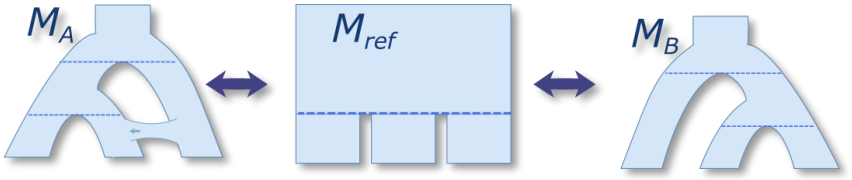
\includegraphics[width=0.8\textwidth]
{A_vs_B_via_ref}
\captionsetup{width=.8\textwidth}
\caption{[TODO - explicitly illustrate how RBFs are used to compare models.]}
\label{fig:model_A__OR__model_b}
\end{figure}



\subsection{The null reference model $\M_0$}

We start by considering a simple case where $\M$ is a demographic model with no migration bands and $\Mref$
is the simplest possible model with a single population of constant size, $\theta_0$.
%
We refer to this simple one-parameter model as the {\em null reference model} (figure \ref{fig:null_model_single_genealogy}). $\M_0$.
%
\begin{figure}[h]
\centering
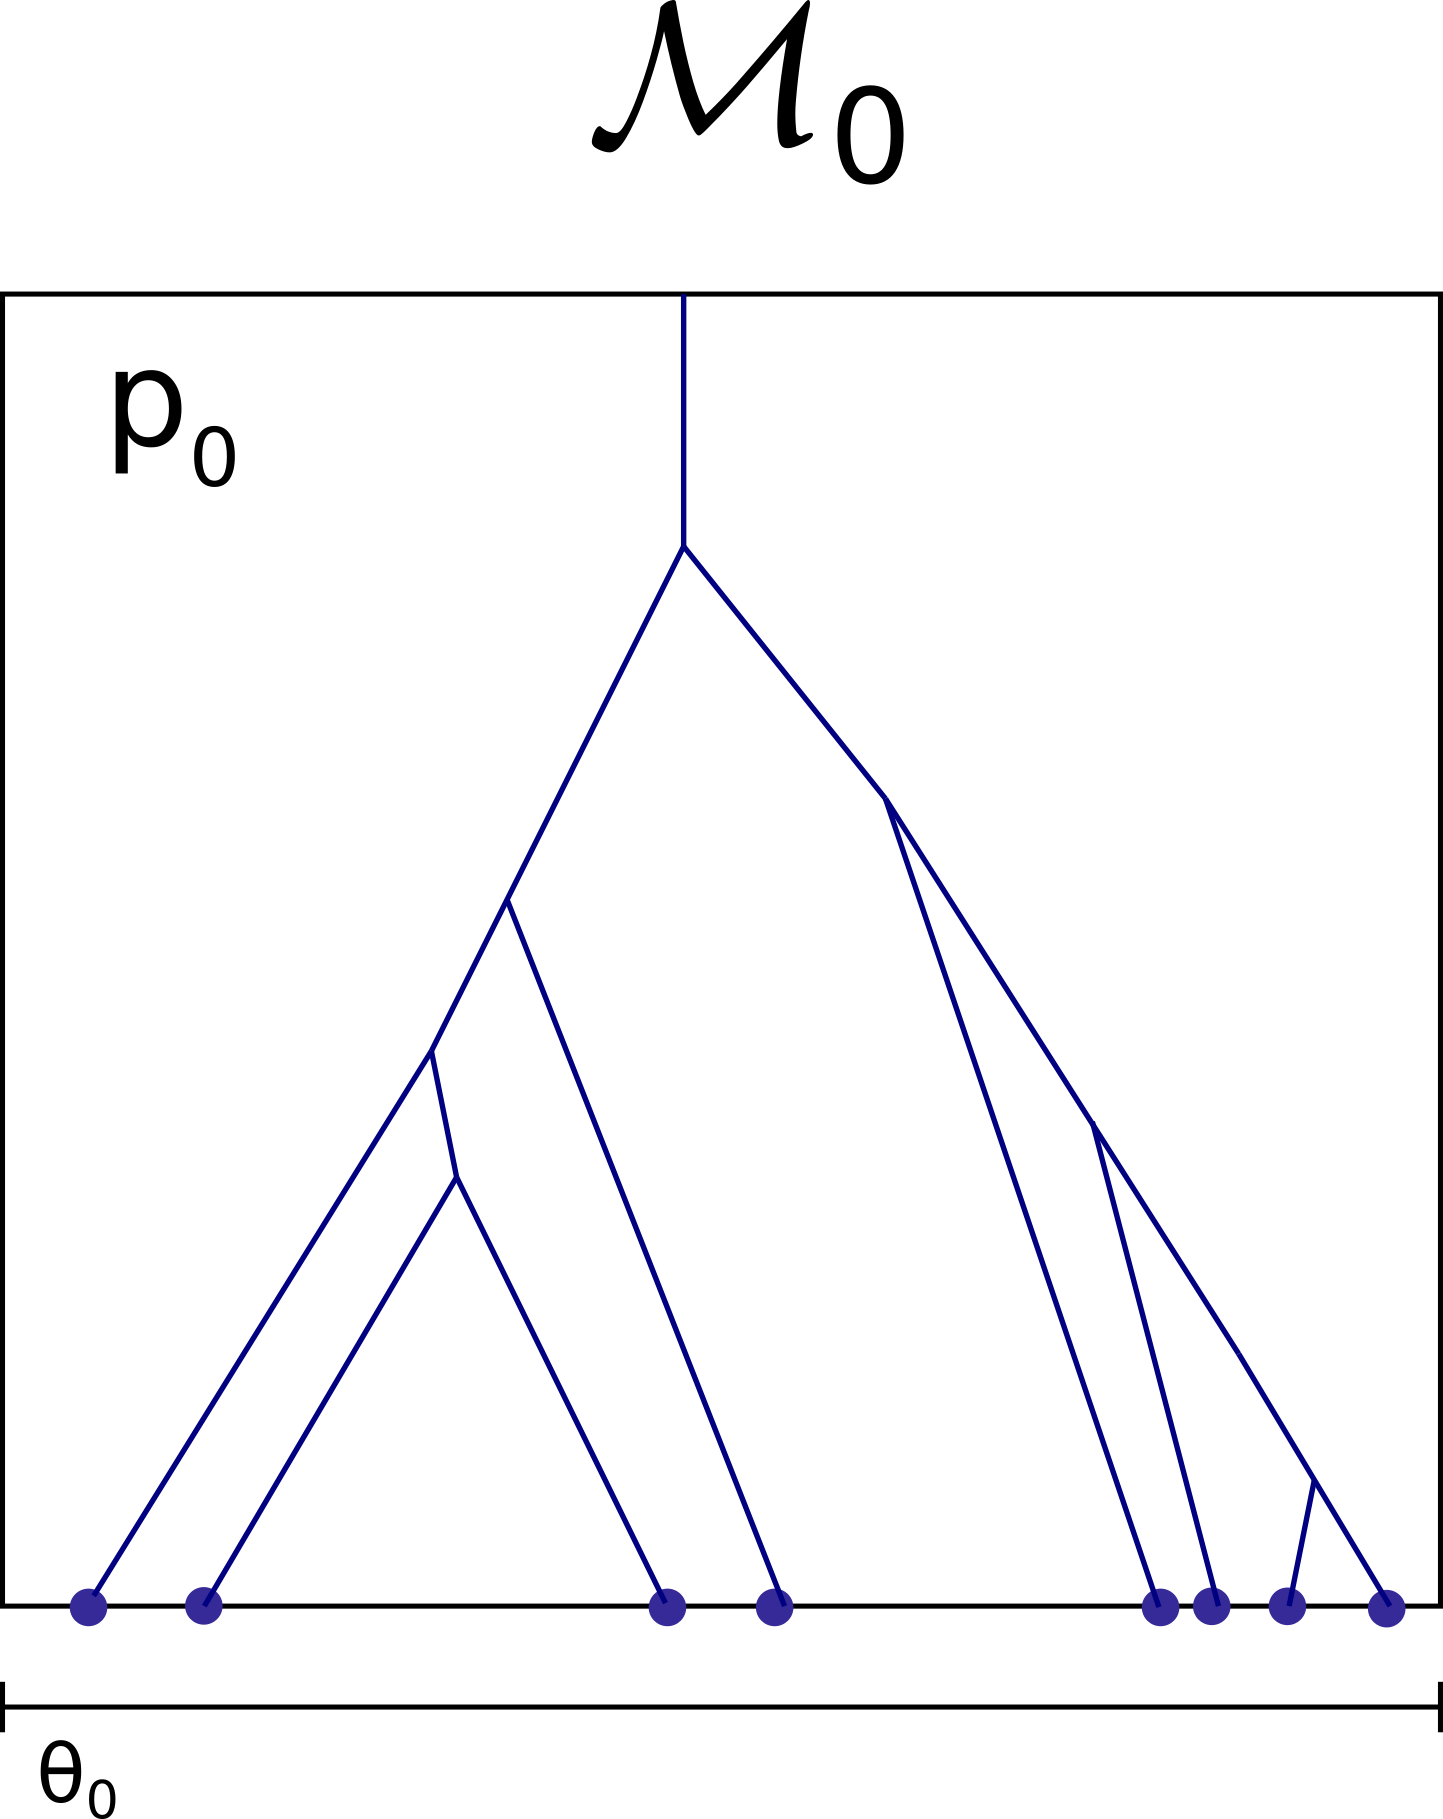
\includegraphics[width=0.3\textwidth]
{null_model_single_genealogy}
\captionsetup{width=.8\textwidth}
\caption{A single local genealogy mapped into the null reference model. The null reference model consists of a single population $p_0$ with $\theta_o := \theta_{root}$. The rest of the free parameters in $\M$ are mapped onto $\M0$ s.t. as many terms as possible terms will cancel-out in the RBF, while meeting conditions (\ref{eq:pref_integral}) \& (\ref{eq:pref_support})n.}
\label{fig:null_model_single_genealogy}
\end{figure}
%
{The first step} of constructing a model-pairing conditional for the two models is to identify a mapping $F$ from the space
of hidden variables in $\M$ to the space of hidden variables in $\M_0$.
%, allowing us to express the likelihood under $\M_0$ as an integral over hidden variables in $\M$.
%
In our case, denote by $\Gref$ and $\Tref$ the hidden variables of $\M_0$.
%
Because both $\M$ and $\M_0$ have no migration bands, then we may assume that the genealogical information used
by both models is the same, implying a natural one-to-one mapping between $\G$ and $\Gref$ (the implications of migration are discussed in the next section).
%
A mapping between $\T=(\taus,\thetas)$ and $\Tref=(\theta_0)$ can be defined by selecting one of the population size parameters in $\T$
to be associated with $\theta_0$. This can be the size of the root population, $\troot$, or any other population
that we expect to best represent the single population in $\M_0$.
%
The model pairing conditional is obtained by applying this mapping and extending it to the unmapped hidden variables, $~ \Z=(\taus,\thetas\setminus \{\troot\})$,
%= \{\tau_p\}\cup\{\theta_p\}_{p\neq root}$,
with the use of a conditional distribution, $\Pref(\Z|\GT\setminus\Z)$:
%
%
\begin{small}
\begin{equation}
 \Pref(\GT|\M_0)  ~~=~~
 P(\theta_0=\troot|\M_0)\ P(\Gref=\G|\M_0,\theta_0=\troot)\ \Pref(\Z|\G,\troot)   ~ .\label{eq:pref_null}
\end{equation}
\end{small}
%
%
The model-pairing condition of Equation \ref{eq:pref_integral} is thus established, regardless of how $\Pref(\Z|\G,\troot)$ is defined:
%
%
\begin{small}
\begin{align}
P(\X|\M_0)
&=~~ \int P(\Tref|\M_0)\ P(\Gref|\M_0,\Tref)\ P(\X|\Gref)\   d\Gref d\Tref  \notag \\ %
&=~~ \int P(\theta_0=\troot|\M_0)\ P(\Gref=\G|\M_0,\theta_0=\troot)\ P(\X|\G)\  d\G d\troot \notag \\ 
&=~~ \int P(\theta_0=\troot|\M_0)\ P(\Gref=\G|\M_0,\theta_0=\troot)\ P(\X|\G)\
\left( \int \Pref(\Z|\G,\troot)\ d\Z \right) d\G d\troot \notag \\ 
%
&=~~ \int P(\theta_0=\troot|\M_0)\ P`(\Gref=\G|\M_0,\theta_0=\troot)\ \Pref(\Z|\G,\troot)\ P(\X|\G)\ d\GT \notag \\ 
&=~~ \int \Pref(\GT|\M_0)\ P(\X|\G)\ d\GT ~. \label{eq:likelihood_null} %
\end{align}
\end{small}

We are left to construct $\Pref(\Z|\G,\troot)$ so that it ensures the model-pairing condition of Equation \ref{eq:pref_support},
and we wish to use the remaining degree of freedom to minimize the variance of the RBF ratio.
%
Equation \ref{eq:pref_support} is guaranteed by constricting $\Pref(\Z|\G,\troot)$ to have zero values whenever $P(\G,\troot,\Z|\M,\X)=0$.
%
Among the unmapped variables $\Z=(\taus,\thetas\setminus \{\troot\})$, the population size parameters $\thetas\setminus \{\troot\}$ do not 
pose any restrictions on the mapped variables $\G,\troot$. This means that Equations \ref{eq:pref_support} is guaranteed regardless of how their marginal distribution is defined.
%
We thus define their conditional probability distribution according to their prior probability in $\M$, to cancel out terms in the RBF ratio and potentially reduce its variance.
%
\begin{small}
\begin{align}
\frac{\Pref(\GT|\M_0) }{P(\GT|\M)}
&=~~ \frac{ P(\theta_0=\troot|\M_0) ~ P(\G|\M_0,\theta_0=\troot) ~ \Pref(\Z|\G,\troot)} {P(\GT|\M)} \notag \\
&=~~ \frac{ P(\G|\M_0,\theta_0=\troot) }{ P(\G|\M,\T)}~ 
     \frac{ P(\theta_0=\troot|\M_0) \prod_{p\neq \troot}\Pref(\theta_p|\G,\troot) }{P(\troot|\M)\prod_{p\neq \troot}P(\theta_p|\M)}~
     \frac{ \Pref(\taus|\G,\thetas)}{P(\taus|\M)} \notag \\
&=~~ \frac{ P(\G|\M_0,\theta_0=\troot) }{ P(\G|\M,\T)}~ 
     \frac{ P(\theta_0=\troot|\M_0)}{P(\troot|\M)}\
     \frac{ \Pref(\taus|\G,\thetas)}{P(\taus|\M)} ~. \label{eq:rbf_null}
\end{align}
\end{small}

Note that if we assume that $\M$ and $\M_0$ use the same prior distribution over $\theta_{root}$ and $\theta_0$ (resp.),
then the middle term in Equation \ref{eq:rbf_null} also cancels out.
%
We cannot similarly define $\Pref(\taus|\G,\thetas)=P(\taus|\M)$, because this may lead to conflicts between divergence times and coalescence times in $\G$, which result in violation of
the model-pairing condition of Equation \ref{eq:pref_support}.
%
Such conflicts occur when a divergence time $\tau_p$ is deeper than the most recent common ancestor
in $\G$ of two individuals that are each a descendant of a different daughter population of population $p$.
%
% Because such a conflict implies that $P(\GT|\M) = 0$, we must also guarantee that $\Pref(\{\tau_p\}|\G)=0$.
%
Thus, the final step of constructing $\Pref(\GT|\Mref)$ is to construct $\Pref(\taus|\G,\thetas)=\Pref(\taus|\G)$ to have zero values whenever $P(\G|\M,\taus,\thetas)=0$.
%
This guarantee is achieved by computing for each $\tau_p$ an upper bound based on the coalescent events in $\G$
and defining $\Pref(\taus|\G)$ as a product of uniform distributions in the feasible ranges of $\taus$
%
(see  Appendix \ref{ap:cond_nomig} for complete derivation and proof).


\subsection{Models with gene flow}

Assume now that the reference model is still the null model, $\M_0$, but the model of interest, $\M$, has a non-empty
set of migration bands, $B$, associated with migration rate parameters, $\migs=\{m_b:b\in B\}$.
%
Migration complicates the mapping between $\M$ and $\M_0$ because the genealogies in $\M$ hold information
about migration events, but the genealogies in $\M_0$ do not.
%
For a sequence of local genealogies $\G$ in $\M$, denote by $\Gc$ the coalescent trees implied by $\G$
and denote by $\Gm$ the information on migration events in $\G$ (locus, timing of event, branch in $\Gc$, source and target populations).
%
%Because the genealogies $\Gref$ in $\M_0$ have no migration events, then t
%There is a natural mapping between $\Gc$ (of $\M$) and $\Gref$ (of $\M_0$) and $P(\X|\Gref) = P(\X|\Gc)$.
Thus, a mapping between the hidden variables of $\M$ ($\Gc,\Gm,\T$) and the hidden variables of $\M_0$ ($\Gref,\theta_0$) can be defined by
mapping $\Gc$ to $\Gref$ and mapping some $\troot\in\T$ to $\theta_0$.
%
Consequently, the set of unmapped hidden variables is $\Z~=~ (\Gm,\taus,\migs,\thetas\setminus\{\troot\})$.
%
This implies a slight modification of the model-pairing conditional specified in Equation \ref{eq:pref_null}:
%
%
\begin{small}
\begin{align}
 \Pref(\GT|\M_0)
 &=~~ 
 %\Pref(\Gc,\troot,\Z|\M_0) ~~=~~
 P(\theta_0=\troot|\M_0)\  P(\Gref=\Gc|\M_0,\theta_0=\troot)\ \Pref(\Z|\Gc,\troot)  ~ .\label{eq:pref_mig}
\end{align}
\end{small}

The model-pairing condition of Equation \ref{eq:pref_integral} can be confirmed  by following a sequence of equalities similar to the ones we derived for 
the scenario without migration (see Equation \ref{eq:likelihood_null}).
%
We are thus left to specify the conditional distribution $\Pref(\Z|\Gc,\troot)$ to ensure that all $\GT$ for which $P(\Gc,\troot,\Z|\M,\X)=0$
also satisfy $\Pref(\Z|\Gc,\troot)=0$.
%
Since the genealogy trees $\Gc$ do not restrict the population size and migration rate parameters, we may define
the conditional probability for these parameters based on their prior probability under $\M$, so that their terms cancel out in the RBF ratio:
%
%
\begin{small}
\begin{align}
\frac{\Pref(\GT|\M_0) }{P(\GT|\M)}
&=~~ \frac{ P(\theta_0=\troot|\M_0) ~  P(\Gref=\Gc|\M_0,\theta_0=\troot) ~ \Pref(\Z|\Gc,\troot) } {P(\GT|\M)} \notag \\
&=~~ \frac{ P(\Gc|\M_0,\theta_0=\troot) }{ P(\Gc,\Gm|\M,\T)}~ 
     \frac{ P(\theta_0=\troot|\M_0) \prod_{p\neq root}\Pref(\theta_p|\Gc,\troot)~\prod_{b}\Pref(m_b|\Gc,\troot) }{P(\troot|\M)\prod_{p\neq\troot}P(\theta_p|\M)~\prod_{b}P(m_b|\M)}~
     \frac{ \Pref(\taus,\Gm|\Gc)}{P(\taus|\M)} \notag \\
&=~~ \frac{ P(\Gc|\M_0,\theta_0=\troot) }{ P(\Gc,\Gm|\M,\T)}~ 
     \frac{ P(\theta_0=\troot|\M_0)}{P(\troot|\M)}\
     \frac{ \Pref(\taus,\Gm|\Gc)}{P(\taus|\M)} ~. \label{eq:rbf_mig}
\end{align}
\end{small}

As in the case without migration, we are left to define the conditional probability distribution over the restricting hidden variables, which are in this case the divergence times
$\taus$ and the migration events $\Gm$.
%
The complex dependence between divergence times and migration events makes this particularly challenging.
%
For instance, a migration event between populations $p_1$ and $p_2$ at time $t$ implies that the divergence times of all populations ancestral to $p_1$ and $p_2$ is at least $t$,
%
but at the same time this migration event may also relax the upper bound of these divergence times.
%
Thus, bounds on divergence times cannot be determined solely based on $\Gc$, and the conditional $\Pref(\taus,\Gm|\Gc)$ cannot be factored into a product of
two separate probability distributions for $\taus$ and $\Gm$.
%
In Appendix \ref{ap:cond_mig} we present a specification for the joint conditional distribution $\Pref(\taus,\Gm|\Gc)$,
which addresses this complex dependence and ensures that $\Pref(\taus,\Gm|\Gc)=0$ whenever $P(\taus,\Gm,\Gc|\M)=0$.
%%
This construction results in additional terms canceling out with terms in  the genealogy likelihood
$P(\Gc,\Gm|\M,\T)$, to further reduce the variance of the RBF ratio.


\subsection{The comb reference model}


The null model has the unique advantage of being a valid reference for the comparison of any two models.
This advantage, however, comes at the cost of collapsing all population structure.
%
In many cases we know the population designation of the sampled individuals, and model uncertainty is restricted to the relationships between the sampled populations.
%
To capture this simple structure we use a population phylogeny with a single ancestral population splitting simultaneously into all sampled populations.
We refer to such models as {\em comb} models and denote them by $\Mcomb$,  due to the comb-like structure of the population phylogeny.
%
A comb model is defined by: (1) a set of sampled (leaf) populations, $L$; (2) an ancestral population, $comb$; and (3) a set of migration bands $B_L$ between populations in $L$.
%
The resulting demographic model, $\Mcomb(L,B_L)$, has $|B_L|+|L|+2$ parameters: $\Tref ~=~ (\tacomb, \widetilde{\thetas},\widetilde{\migs})$,
where $\widetilde{\thetas}=\{\theta_p:p\in L\cup \{comb\}\}$ and $\widetilde{\migs} = \{m_b:b\in B_L\}$.
%

\begin{figure}[h]
\centering
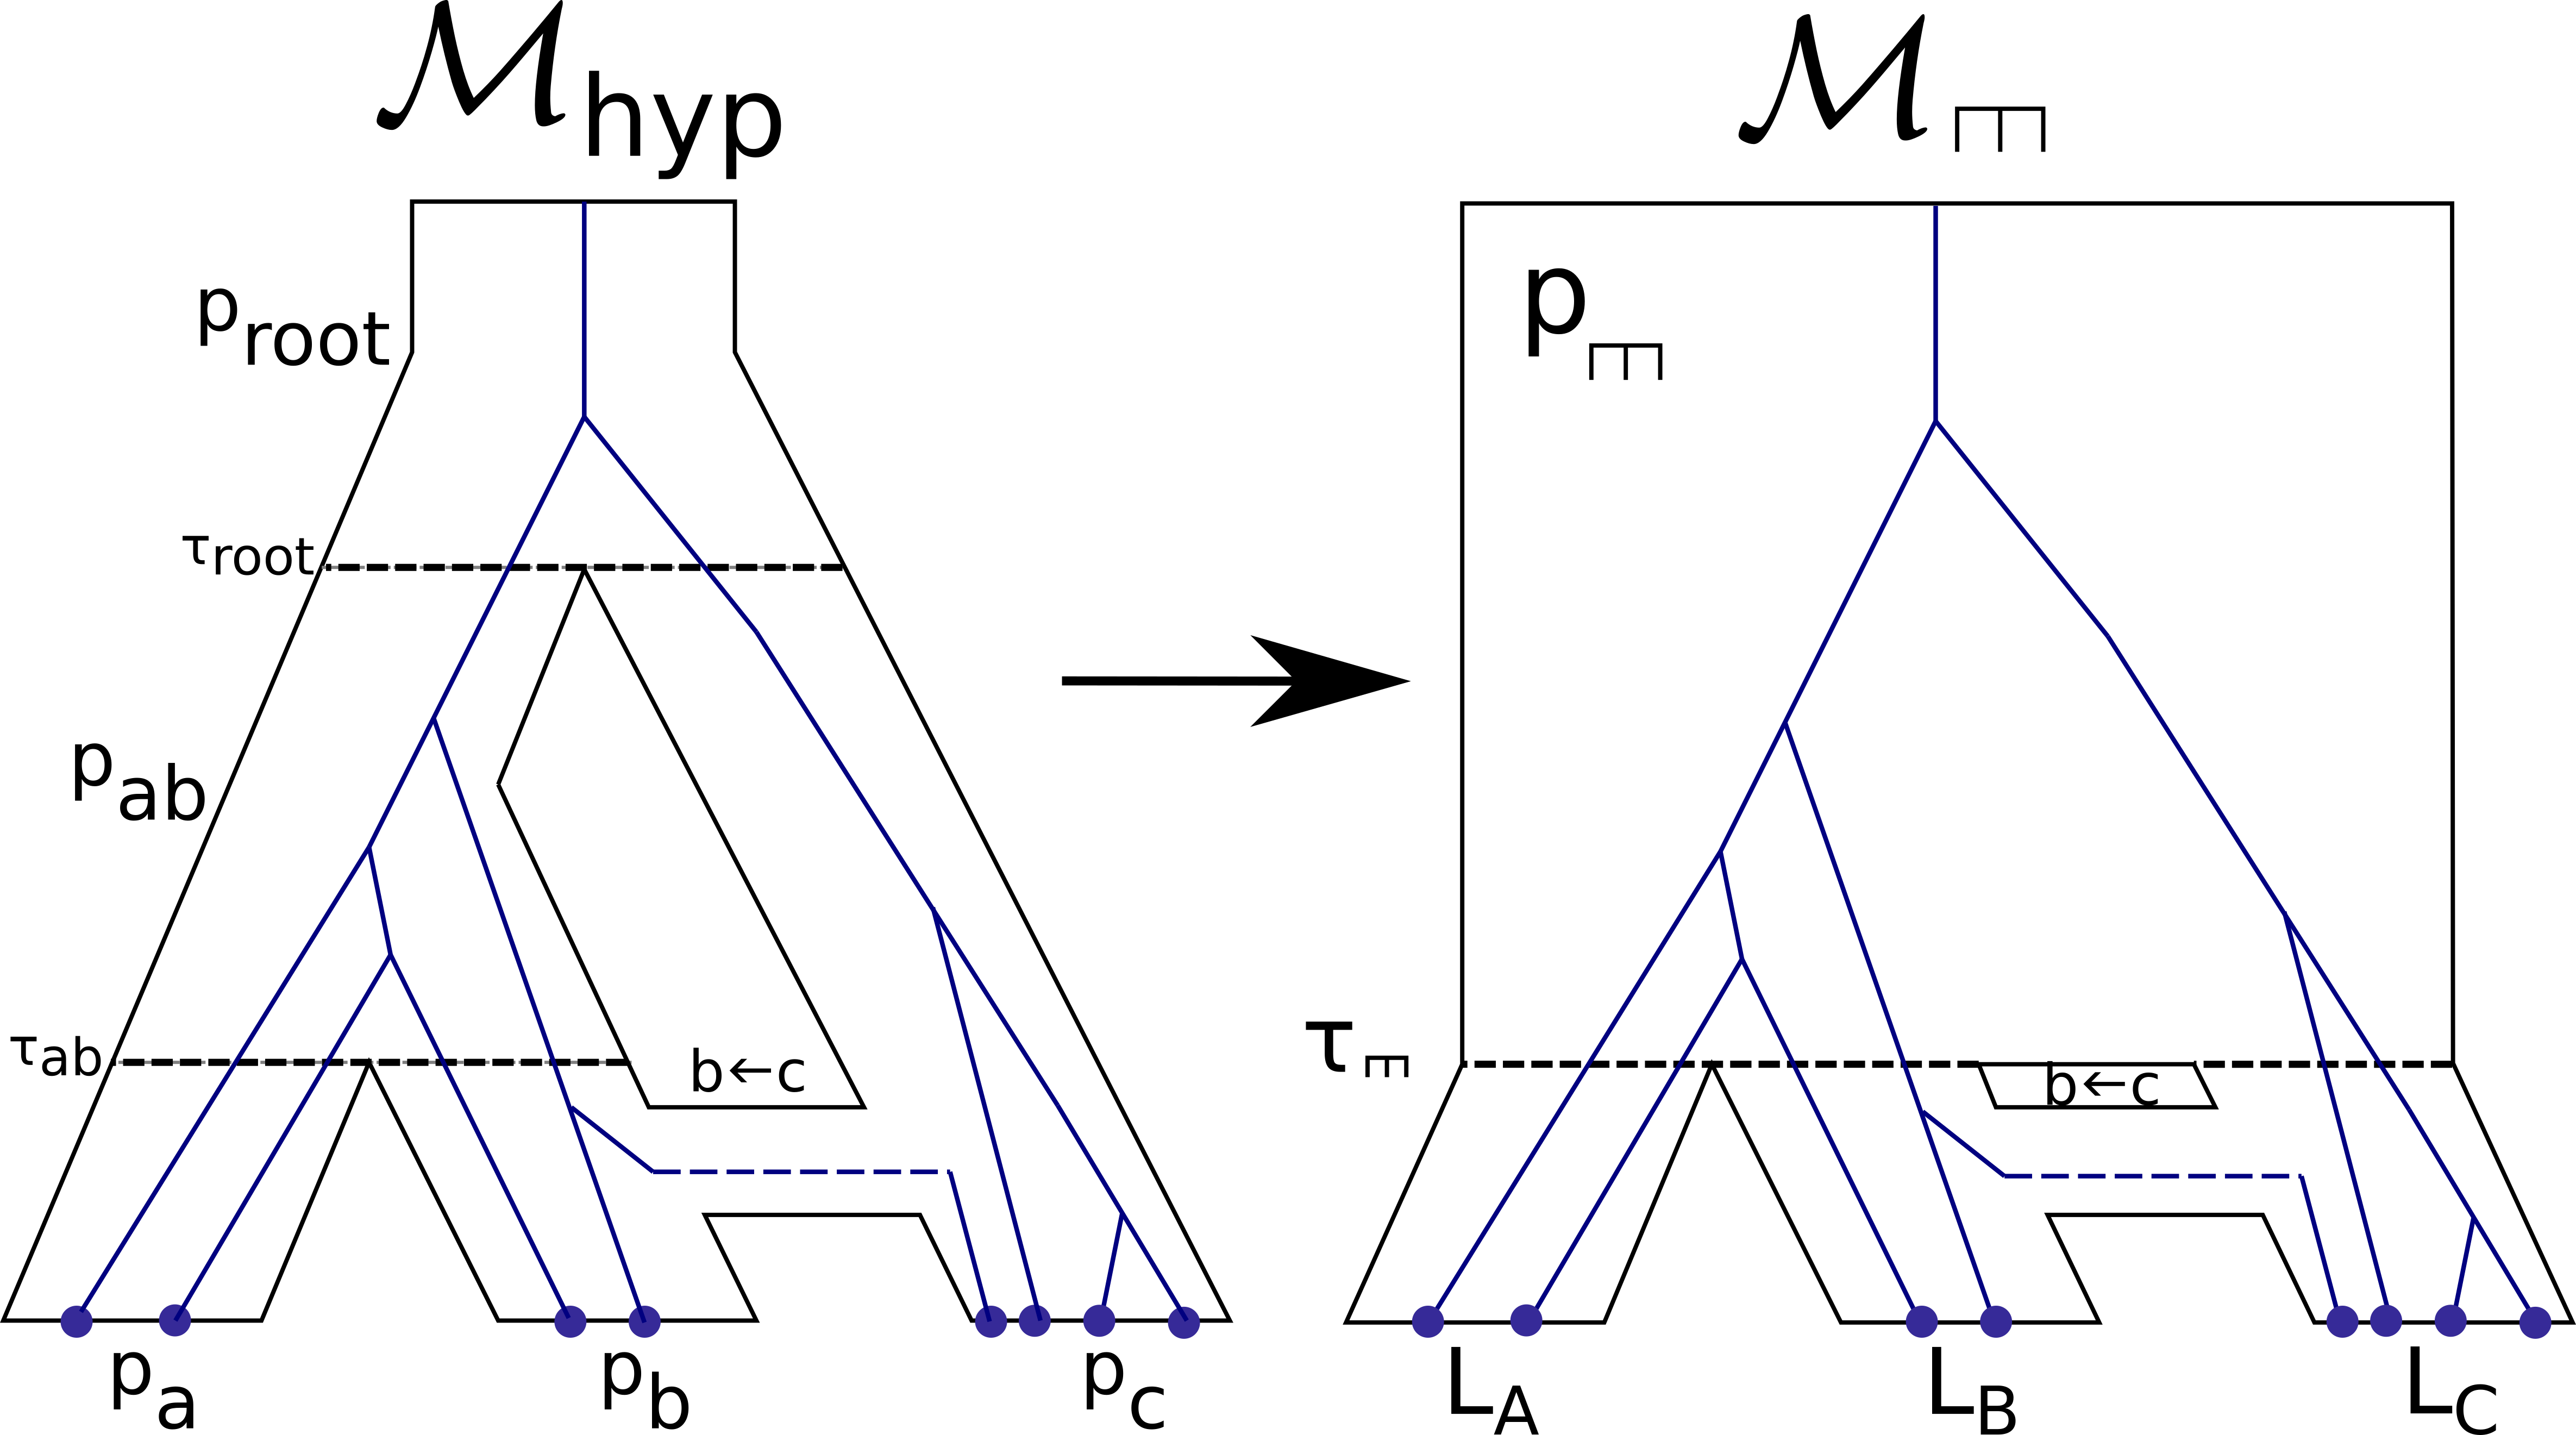
\includegraphics[width=0.4\textwidth]
{comb_model_single_genealogy}
\captionsetup{width=.8\textwidth}
\caption{A single local genealogy mapped into the comb reference model. The comb model consists of a single ancestral population $p_{comb}$ [TODO - use $p$ with the comb symbol instead of $p_{comb}$ ] which splits simultaneously into leaves $L$.}
\label{fig:comb_model_single_genealogy}
\end{figure}


%
Consider a demographic model, $\M(\Tr,B)$, and its corresponding comb model, $\Mcomb(L,B_L)$, defined by $L=leaves(\Tr)$ and $B_L=B \cap (L \times L)$.
%
For brevity, we refer to $\Mcomb(L,B_L)$ simply as $\Mcomb$.
%
The model-pairing conditional distribution for $\M$ and $\Mcomb$ is constructed by first defining a mapping between the hidden variables of $\M$ ($\GT$) and the hidden variables of $\Mcomb$ ($\Gref\Tref$).
%
This mapping is derived from the requirement that below the comb divergence time ($\tacomb$) the comb model is identical to $\M$ and above it $\Mcomb$ is identical to the null model $\M_0$.
%
We thus set $\tacomb=\tmin\eqdef\min(\taus)$, to guarantee that all population divergence events in $\M$ map to the comb population in $\Mcomb$.
%
The migration rates of bands in $\B \cap (L \times L)$ and effective sizes of populations in $L$ are mapped into their counterparts in $\Tref$,
%
and following the mapping for the null model, a single ancestral population size parameter ($\troot$) is chosen to be mapped into $\thcomb$.
%
We denote the set of mapped migration rate and population size parameters of $\M$ collectively as $\Tcomb$.
%
Mapping between genealogies is obtained by {removing from $\G$ all migration events above time $\tmin$}.
The resulting collection of local genealogies are denoted by $\Gcomb$ and are directly mapped to $\Gref$.
%
The remaining unmapped hidden variables ($\Z$) of $\M$ consist of the following components:
\begin{enumerate}
 \item Unmapped population size parameters: $\{\theta_p : p\notin L\cup \{root\}\ \}$.
 \item Unmapped migration rate parameters:  $\{m_b: b\notin L \times L \}$.
 \item The identity of the ancestral population in $\Tr$ with minimum divergence time: $minAncPop=\argmin(\taus)$. 
   Note that this population may be \emph{any ancestral population with two leaf daughters}, and its identity is lost when mapping $\taus$ into $\tacomb$.
 \item The divergence times of all other populations: $\{\tau_p:p\neq minAncPop\}$.
 \item Information on all migration events in $\G$ above time $\tacomb$, which we denote by $\G_{m|>\tmin}$.
\end{enumerate}


A model-pairing conditional distribution for $\M$ and $\Mcomb$ is thus established by applying the mapping described above and
specifying a conditional distribution over the unmapped parameters, $\Pref(\Z|\Gcomb,\Tcomb,\tmin)$. The proof of the condition in Equation \ref{eq:pref_integral} is given below:
%
%
\begin{small}
\begin{align}
 \Pref(\GT|\Mcomb)
 &=
 P(\Tref=(\Tcomb,\tmin)|\Mcomb)\ P(\Gref=\Gcomb|\Mcomb,\Tcomb,\tmin)\ \Pref(\Z|\Gcomb,\Tcomb,\tmin)  ~ .\label{eq:pref_comb}\\
%\notag \\
%\end{align}
%\end{small}
%
%
%\begin{small}
%\begin{align}
P(\X|\Mcomb)
&= \int P(\Tref|\Mcomb)\ P(\Gref|\Mcomb,\Tref)\ P(\X|\Gref)\   d\Gref\Tref  \notag \\ %
&= \int P(\Tref=(\Tcomb,\tmin)|\Mcomb)\ P(\Gref=\Gcomb|\Mcomb,\Tcomb,\tmin)\ P(\X|\Gcomb)\  ~ d\Gcomb\Tcomb\tmin \notag \\ 
&= \int P(\Tref=(\Tcomb,\tmin)|\Mcomb)\ P(\Gref=\Gcomb|\Mcomb,\Tcomb,\tmin)\ P(\X|\Gcomb) \left( \int \Pref(\Z|\Gcomb,\Tcomb,\tmin) d\Z \right) d\Gcomb\Tcomb\tmin \notag \\ 
&= \int P(\Tref=(\Tcomb,\tmin)|\Mcomb)\ P(\Gref=\Gcomb|\Mcomb,\Tcomb,\tmin)\ \Pref(\Z|\Gcomb,\Tcomb,\tmin)\ P(\X|\G)\   d\GT \notag \\ 
&= \int \Pref(\GT|\M_0)\ P(\X|\G)\ d\GT ~. \label{eq:likelihood_comb} %\\
%\notag \\
\end{align}
\end{small}

The conditional distribution $\Pref(\Z|\Gcomb,\Tcomb,\tmin)$ is defined similar to its specification in the null model.
%
The unmapped population size and migration rate parameters are distributed according to their prior probability under $\M$ to eliminate terms in the RBF ratio.
%
The identity of the minimal ancestral population, $minAncPop$, is distributed uniformly among all ancestral populations in $\Tr$ with two leaf daughters.
%
We denote the number of such populations in $\Tr$ by $\kappa(\Tr)$.
%
The only unmapped variables restricted by $\Gcomb$ and $\tmin$ are the unmapped divergence times and migration events above time $\tmin$. Their conditional distribution,
$\Pref(\taus\setminus\{\tmin\},\G_{m|>\tmin}|\Gc)$, is defined using the process described for the null model (see Appendices \ref{ap:cond_nomig} and \ref{ap:cond_mig}).
%
This specification thus guarantees the condition of Equation \ref{eq:pref_support}, as in the case of the null reference model.
%
The resulting RBF ratio is expressed as follows:
%
%
\begin{small}
\begin{align}
\frac{\Pref(\GT|\Mcomb) }{P(\GT|\M)}
&= \frac{ P(\Tref=(\Tcomb,\tmin)|\Mcomb) ~ P(\Gref=\Gcomb|\Mcomb,\Tcomb,\tmin) ~ \Pref(\Z|\Gcomb,\Tcomb,\tmin) } {P(\GT|\M)} \notag \\
&= \frac{ P(\Gref=\Gcomb|\Mcomb,\Tcomb,\tmin) }{ P(\G|\M,\T)}~ 
   \frac{ P(\Tref=(\Tcomb,\tmin)|\Mcomb) }{ P(\Tcomb|\M) }~
   \frac{ \frac{1}{\kappa(\Tr)}\Pref(\taus\setminus\{\tmin\},\G_{m|>\tmin}|\Gc)}{P(\taus|\M)} ~. \label{eq:rbf_comb}
\end{align}
\end{small}


As in the case of the null reference model, the above RBF ratio has several terms canceling out. First, the conditional probabilities of the unmapped population size and
migration rate parameters cancel out with their priors under $\M$. Second, if we assume identical priors in both models for the mapped parameters,
then these cancel out as well in the second term of Equation \ref{eq:rbf_comb}.
Terms in the genealogy likelihood contributed by migration events above time $\tmin$ also cancel out in the ratio (see Appendix \ref{ap:cond_mig}).
Finally, the contribution of all events below time $\tmin$ (coalescence and migration) also cancel out.
If we denote the portion of $\G$ below time $\tmin$ by $\G_{<\tmin}$, and the portion above it by $\G_{>\tmin}$, then the contribution of $\G_{<\tmin}$ 
to the first term of the RBF ratio cancels out as follows:
%
%
\begin{small}
\begin{align}
\frac{ P(\Gcomb|\Mcomb,\Tcomb,\tmin) }{ P(\G|\M,\T)}
&=~~ \frac{ {P(\Gcomb}_{<\tmin}|\Mcomb,\Tcomb,\tmin) P({\Gcomb}_{>\tmin}|\Mcomb,\Tcomb,\tmin) }{ P(\G_{<\tmin}|\M,\T) P(\G_{>\tmin}|\M,\T)}   \notag \\
&=~~ \frac{ {P(\G}_{<\tmin}|\Mcomb,\Tcomb,~\tacomb=\tmin)}{ P(\G_{<\tmin}|\M,\Tcomb,~\min(\taus)=\tmin)} ~\frac{ P({\G}_{c|>\tmin}|\Mcomb,\thcomb=\troot) }{ P(\G_{>\tmin}|\M,\T)}   \notag \\
&=~~ \frac{ P({\G}_{c|>\tmin}|\M_0,\theta_0=\troot) }{ P(\G_{>\tmin}|\M,\T)} ~.  \label{eq:gen_ratio_comb}
\end{align}
\end{small}

The RBF may thus be re-expressed as follows:
%
%
\begin{small}
\begin{align}
\frac{\Pref(\GT|\Mcomb) }{P(\GT|\M)}
&= \frac{1}{\kappa(\Tr)} ~
   \frac{\Pref(\G_{>\tmin},\ \T\setminus\{\tmin\}\ |\ \M_0) }{P(\G_{>\tmin},\ \T\setminus\{\tmin\}\ |\ \M)} ~
   \frac{ P(\Tref\setminus\{\thcomb\}=(\Tcomb\setminus\{\troot\},\tmin)|\Mcomb) }{ P(\Tcomb\setminus\{\troot\}|\M) }~. \label{eq:rbf_comb1}
\end{align}
\end{small}



\subsection{Constructing a Reference Model}  \label{Constructing a Reference Model}

In many cases of interest, the modeling uncertainty is restricted to a certain subtree in the population phylogeny.
%
In such cases, we wish to consider a reference model where only a subset of the sampled populations $P$ is collapsed into a single clade population, or a comb model. The null and comb models discussed above are special cases where
$P$ is the entire set of sampled populations.\\
%
In general describe, a reference model $\Mref$ for hypothesis model $\M$ may be obtained by applying the following three-step process:

\begin{enumerate}
\item First, \textbf{choose a subtree} of the population phylogeny of $\M$. The subtree is associated with the population $p$ at its root. 

\item Then \textbf{collapse the subtree structure} into either a clade structure, i.e. a single population $p_{clade}$ (figure (\ref{fig:clade_collapse_AB})), or a comb structure, i.e. an ancestral population $p_{comb}$ [TODO - use good comb annotation] and a set of leaf populations and migration bands $L, B_L$. 

\item Finally, \textbf{map the hidden parameters} of $\M$ onto parameters of $\Mref$, defining the model-pairing conditional distribution $\Pref$ s.t. conditions (\ref{eq:pref_integral}) and (\ref{eq:pref_support}) are met. This mapping should cancel-out as many terms of the RBF ratio as possible (equations (\ref{eq:rbf_mig}) \& (\ref{eq:rbf_comb1})).
\end{enumerate}

Identically mapping all structure and parameters outside the subtree of $p$ during step 3 leads to canceling-out of all corresponding terms in the RBF of $\M$ relative to $\Mref$.

%
\begin{figure}[h]
\centering
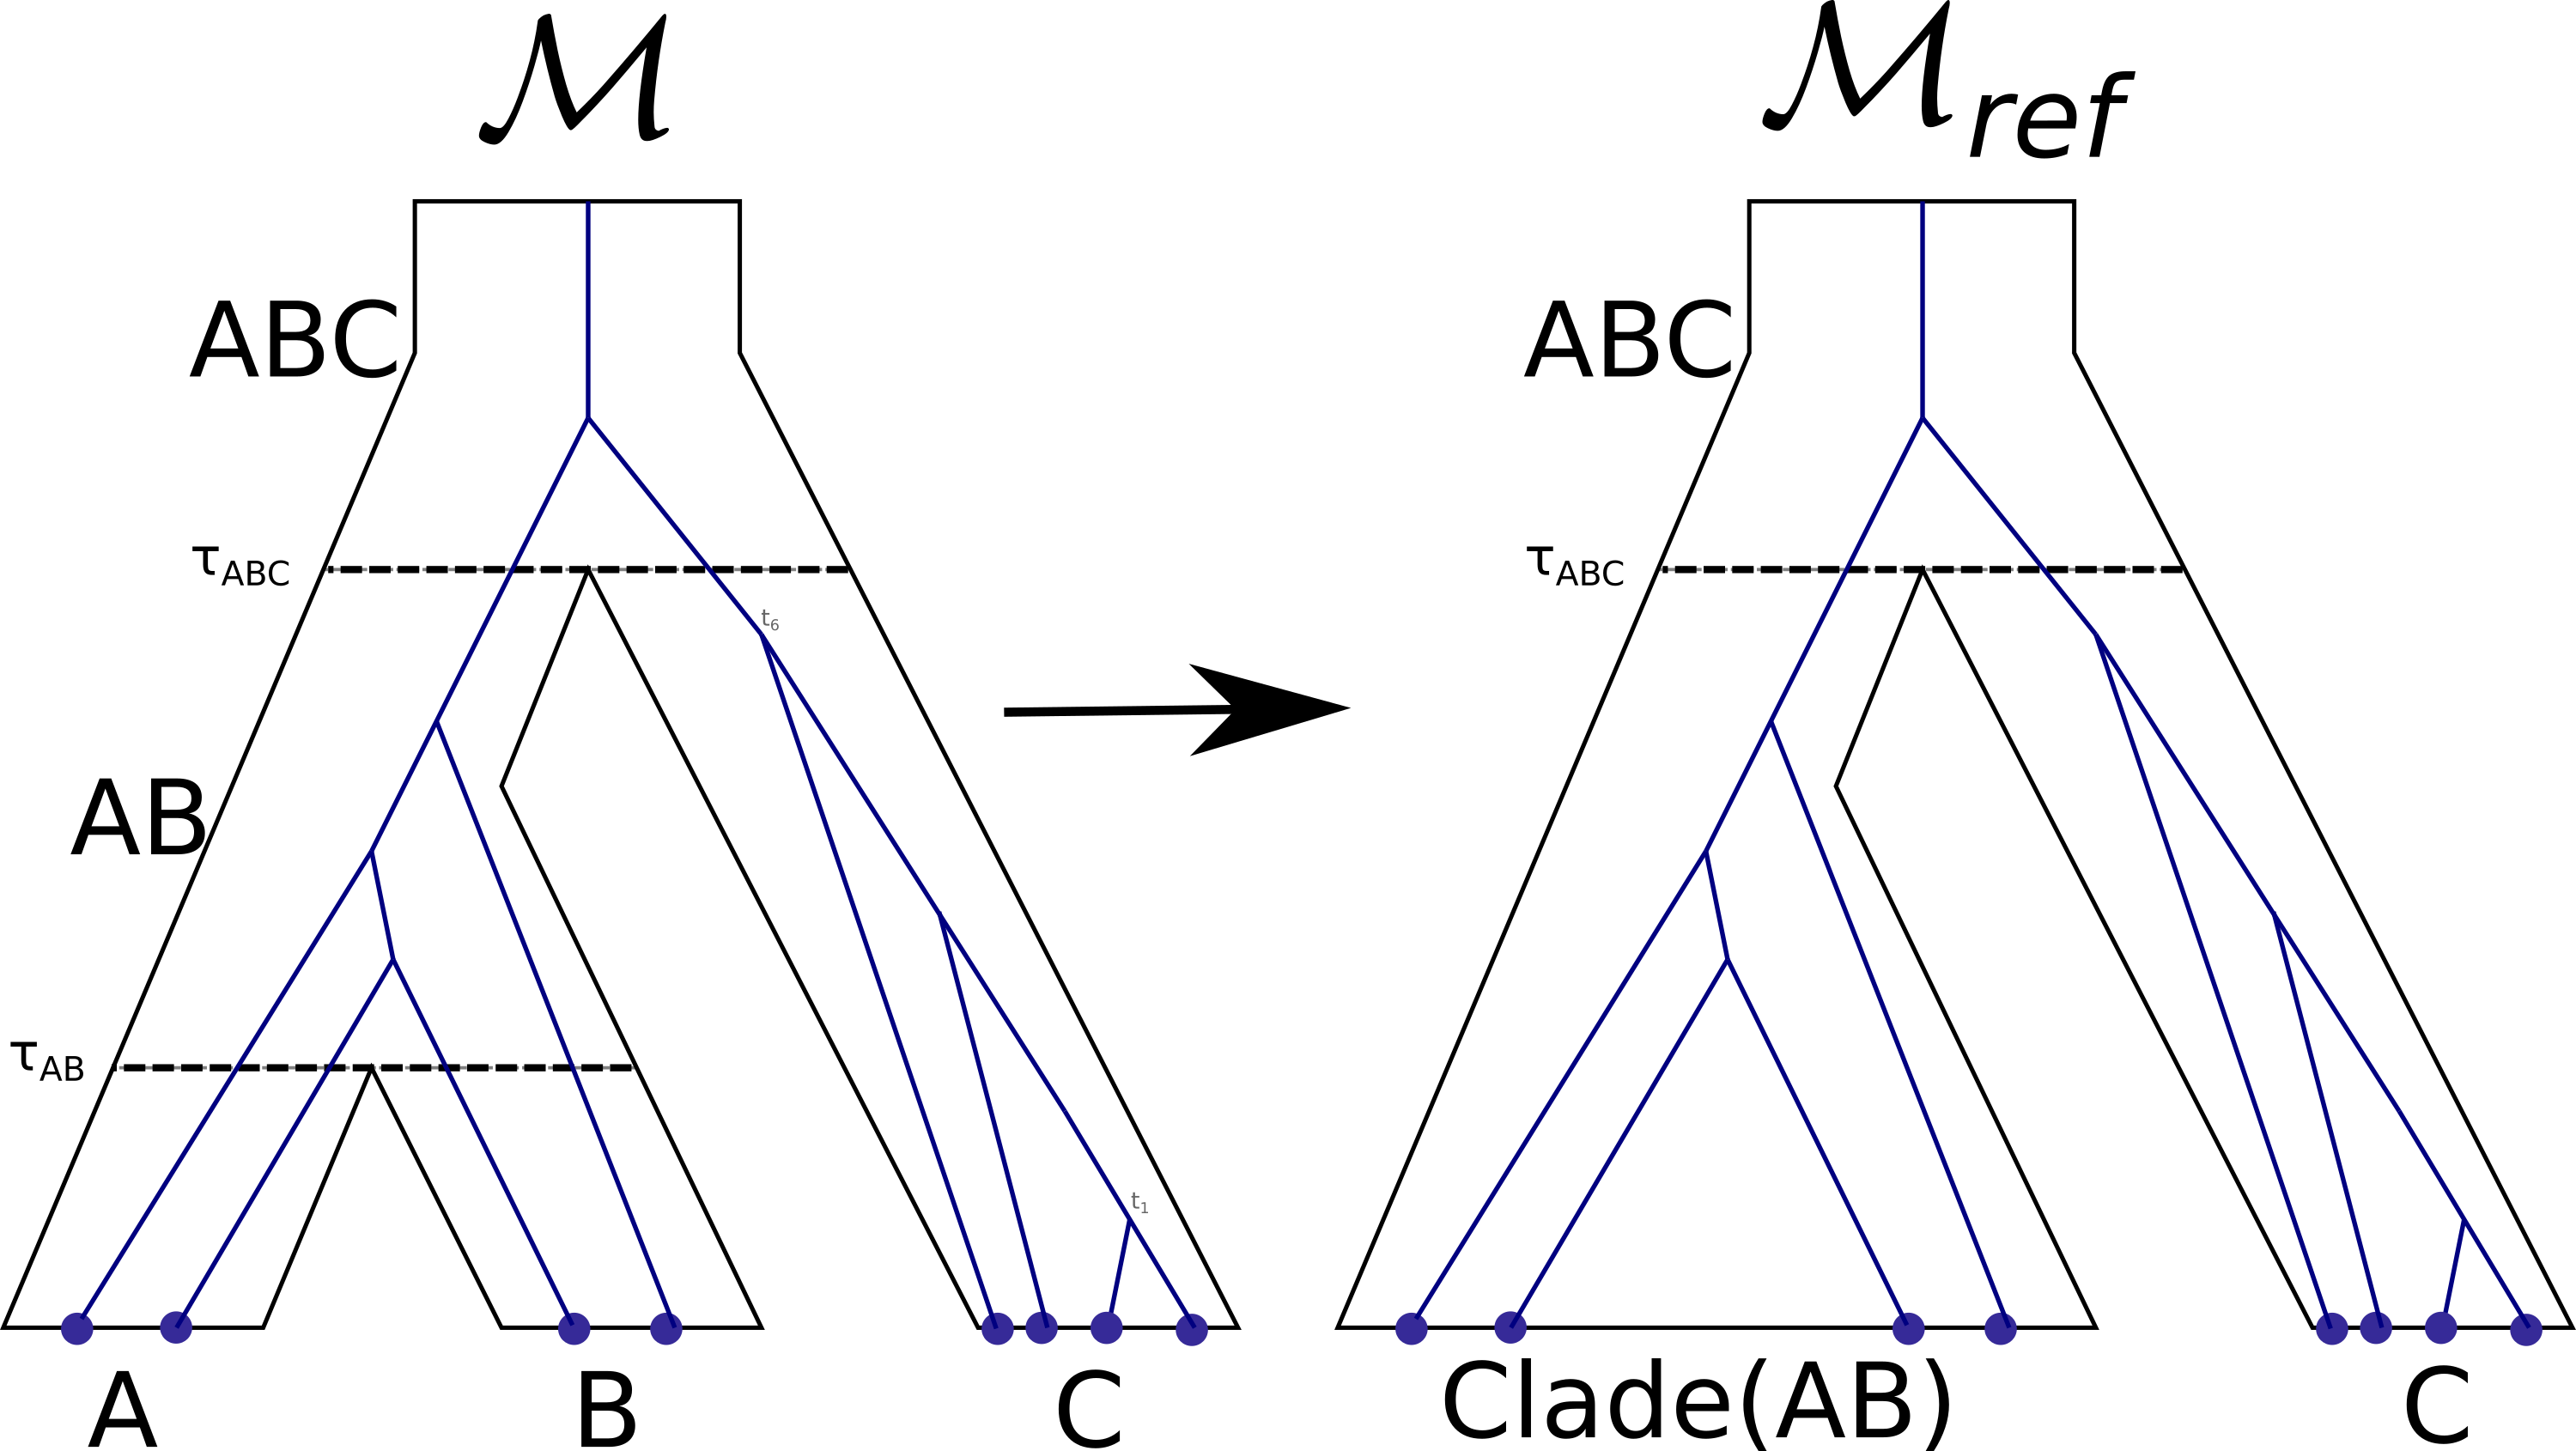
\includegraphics[width=0.8\textwidth]
{clade_collapse_AB}

\captionsetup{width=.8\textwidth}
\caption{\textbf{Construction of a reference model via clade-collapse - } The reference model  $\Mref$ is created by clade-collapsing  the subtree rooted at $AB$ and identically mapping the rest of the hypothesis. Genealogy and paramter likelihoods pertaining to populations $ABC$ and $C$ will cancel-out in the RBF formula. [TODO - color the populations that get collapsed] [TODO - move arrow to middle between models. increase font size of taus]}
\label{fig:clade_collapse_AB}
\end{figure}


\section{Calculations Schema}

Having formulated the RBF and defined reference models and their use, we now move on to expain in detail how the model-comparison criteria are calculated.

\subsection{The Computational Objective}

Consider formula (\ref{eq:rbf}) for calculating the Bayes Factor of model $M$ relative to $\Mref$:
%
%
\begin{equation}
 \frac{1}{\rbf(\M:\Mref|\X)} ~~\triangleq~~ ...  ~~\approx~~ \frac{1}{N} \sum_{i=1}^{N}\frac{\Pref(\GT^{(i)}|\Mref) }{P(\GT^{(i)}|\M)} ~ 
 \notag
\end{equation}

Since the denominator $P(\GT^{(i)}|\M)$ is constantly calculated by \gp in the MCMC process, what remains for mcref to calculate in order to estimate the Bayes Factor is the model pairing conditional $\Pref(\GT^{(i)}|\Mref)$. The following chapter addresses efficient calculation of the genealogy likelihood, since it is the main component making up the model pairing conditional and represents the bulk of our computational challenge.\\


\subsection{Efficient Sufficient Statistics for Reference Model Genealogy Likelihood}


We note that there exists a natural trade-off between the flexibility in choice of reference model and the amount of data the MCMC process is required to emit. For example, if no flexibility is required and the reference model is predetermined before MCMC execution, formula (9) can be calculated during MCMC iteration and only the final RBF value need be emitted. However, calculating (9) on any other reference model would require another full MCMC run.
%
On the other hand, the RBF for every reference model can be computed in post-processing if the MCMC prints out the full hidden state $\GT$ in each iteration.
%
However this would yield an unreasonable amount of traced information, in proportion to the size of the model and to the number of loci.


We designed a computational scheme that aims to find a reasonable middle ground between these two extreme options.
Our objective was to maximize the number of reference models we could consider after running a single MCMC sampling chain without blowing up the output trace.
This is done by identifying a collection of sufficient statistics for $\G$ that satisfy two conditions:
%
%
\begin{enumerate}
 \item The number of sufficient statistics depends on the complexity of the target model, $\Mref$, but not on the size of the data (i.e. the number of individuals and the number of loci).
 \item The sufficient statistics allow calculation of $P(\G|\T,\Mref)$ for a wide variety of reference models and values of model parameters (namely, migration rates and population sizes).
\end{enumerate}
%

Sufficient statistics that satisfy these conditions are derived from the expression for the genealogy likelihood $P(\G|\T, \Mref)$ under Kingman's coalescent, which we briefly recall here.
First, because the loci are assumed to be freely recombining, then the local genealogies $\G=(G_1,...G_L)$ are conditionally independent given the model parameters and the likelihood may be expressed as a product of locus-specific likelihoods, $P(G_l|\T,\Mref)$.  Each locus-specific likelihood is a product of exponentially distributed waiting times for coalescent and migration events. The rates of these exponential distributions depend on the model parameters (population sizes and migration rates) as well as the number of lineages considered for coalescence and migration. We thus identify for each population the set of coalescent and migration events that change the number of lineages modeled in that population in $G_l$. Each time interval $I$ between two consecutive events is associated with the following properties:
\begin{itemize}
 \item $t(I)$ -- the elapsed time of the interval.
 \item $n(I)$ -- the number of lineages of $\G_l$ alive during that time in the target population.
 \item $isCoal(I)$ , $isInMig(I)$  -- binary values that indicate whether the event above the interval is a coalescent event or incoming migration event (respectively).
\end{itemize}
%
%
The contribution of population $p$ to $P(G_l|\T,\Mref)$ can then be expressed as a product over the set of relevant time intervals $\Ip$:
%
%
\begin{small}
\begin{align}
f_{coal}(\G_l,p|\T,\Mref) 
& ~\triangleq~ \prod_{I \in \Ip} \left(\frac{2}{\theta_p}\right)^{isCoal(I)} \exp\left(-\frac{2}{\theta_p}{n(I) \choose 2}t(I)\right) ~. %\notag\\
% & ~=~ \left(\frac{2}{\theta_p}\right)^{numCoals(G_l,p)} \exp\left( -\frac{1}{\theta_p} \sum_{I \in \Ip} (n(I)^2-n(I))~t(I) \right) ~.
\label{eqn:ld-coal}
\end{align}
\end{small}
%
%
Similarly, the contribution of migration band $b$ to $P(G_l|\T,\Mref)$ can be expressed as a product over the set of time intervals $\Ib$ defined by events in the target population of the migration band:
%
%
\begin{small}
\begin{equation}
f_{mig}(\G_l,b|\T,\Mref) ~\triangleq~ \prod_{I \in \Ib} m_{b}^{isInMig(I)} ~ \exp \left( - m_b~ n(I)~t(I)\right) ~.
\label{eqn:ld-mig}
\end{equation}
\end{small}
%
%

Using these notations, the genealogy log likelihood can be expressed as follows:
%
%
\begin{small}
\begin{align}
\ln \left( P(\G| \T,\Mref) \right) ~&=~ \ln \left( \prod_{l}  P(G_l| \T,\Mref) \right)  \notag \\ 
%
&=~  \ln \left( ~\prod_{l}  \left( \prod_{p} f_{coal}(\G_l,p|\T,\Mref) ~ \prod_{b} f_{mig}(\G_l,b|\T,\Mref) \right) ~\right) \notag \\ 
%
&=~  \sum_{p}\sum_{l}\ln \left( f_{coal}(\G_l,p|\T,\Mref) \right) ~ + ~ \sum_{b}\sum_{l}\ln \left( f_{mig}(\G_l,b|\T,\Mref) \right)~. 
\label{eqn:ld-details}
\end{align}
\end{small}

The key to likelihood calculation is to sum over the log-likelihood contributions across time intervals and across loci (see figure \ref{fig:multiple_loci}):
%
%
\begin{small}
\begin{align}
\sum_{l}\ln \left( f_{coal}(\G_l,p|\T,\Mref) \right) &=~ %\sum_{l} \sum_{I \in \Ip} \left( isCoal(I)\cdot \ln \left( \frac{2}{\theta_p}\right)~-~\frac{(n(I)^2-n(I))~t(I)}{\theta_p} \right)\notag \\
%&=~ 
\ln\left( \frac{2}{\theta_p}\right) \sum_{l} \sum_{I \in \Ip} isCoal(I)  - \frac{2}{\theta_p} \sum_{l} \sum_{I \in \Ip}{n(I)\choose 2}t(I) ~.
\label{eqn:ld-coal-stats}\\
% &\notag\\
\sum_{l}\ln \left( f_{mig}(\G_l,b|\T,\Mref) \right) &=~ %\sum_{l} \sum_{I \in \Ib} \left( isInMig(I)\cdot \ln\left( m_b\right) ~-~ m_b n(I) t(I) \right) \notag \\
%&=~
\ln\left( m_b\right) \sum_{l} \sum_{I \in \Ip} isInMig(I)  - m_b \sum_{l} \sum_{I \in \Ip}n(I) t(I) ~.
\label{eqn:ld-mig-stats}
\end{align}
\end{small}

Note that the four double sums in these expressions depend on the local genealogies $\G$ and the divergence times $\{\tau_p\}$, but they do not depend on the population size and migration rate parameters. We thus denote these sums respectively as $numCoals(\G,p)$, $coalStats(\G,p)$,  $numMigs(\G,b)$, and $migStats(\G,b)$, and the log-likelihood can be expressed as follows:
%
%
\begin{small}
\begin{align}
\ln \left( P(\G| \T,\Mref) \right) ~=&~ \sum_{p}  \ln\left( \frac{2}{\theta_p}\right)\cdot numCoals(\G,p) - \frac{1}{\theta_p}\cdot coalStats(\G,p) \\
& +~ \sum_{b}  \ln\left( m_b\right)\cdot numMigs(\G,b) - m_b \cdot migStats(\G,b) ~. 
\label{eqn:ld-final}
\end{align}
\end{small}


\begin{figure}[h]
\centering
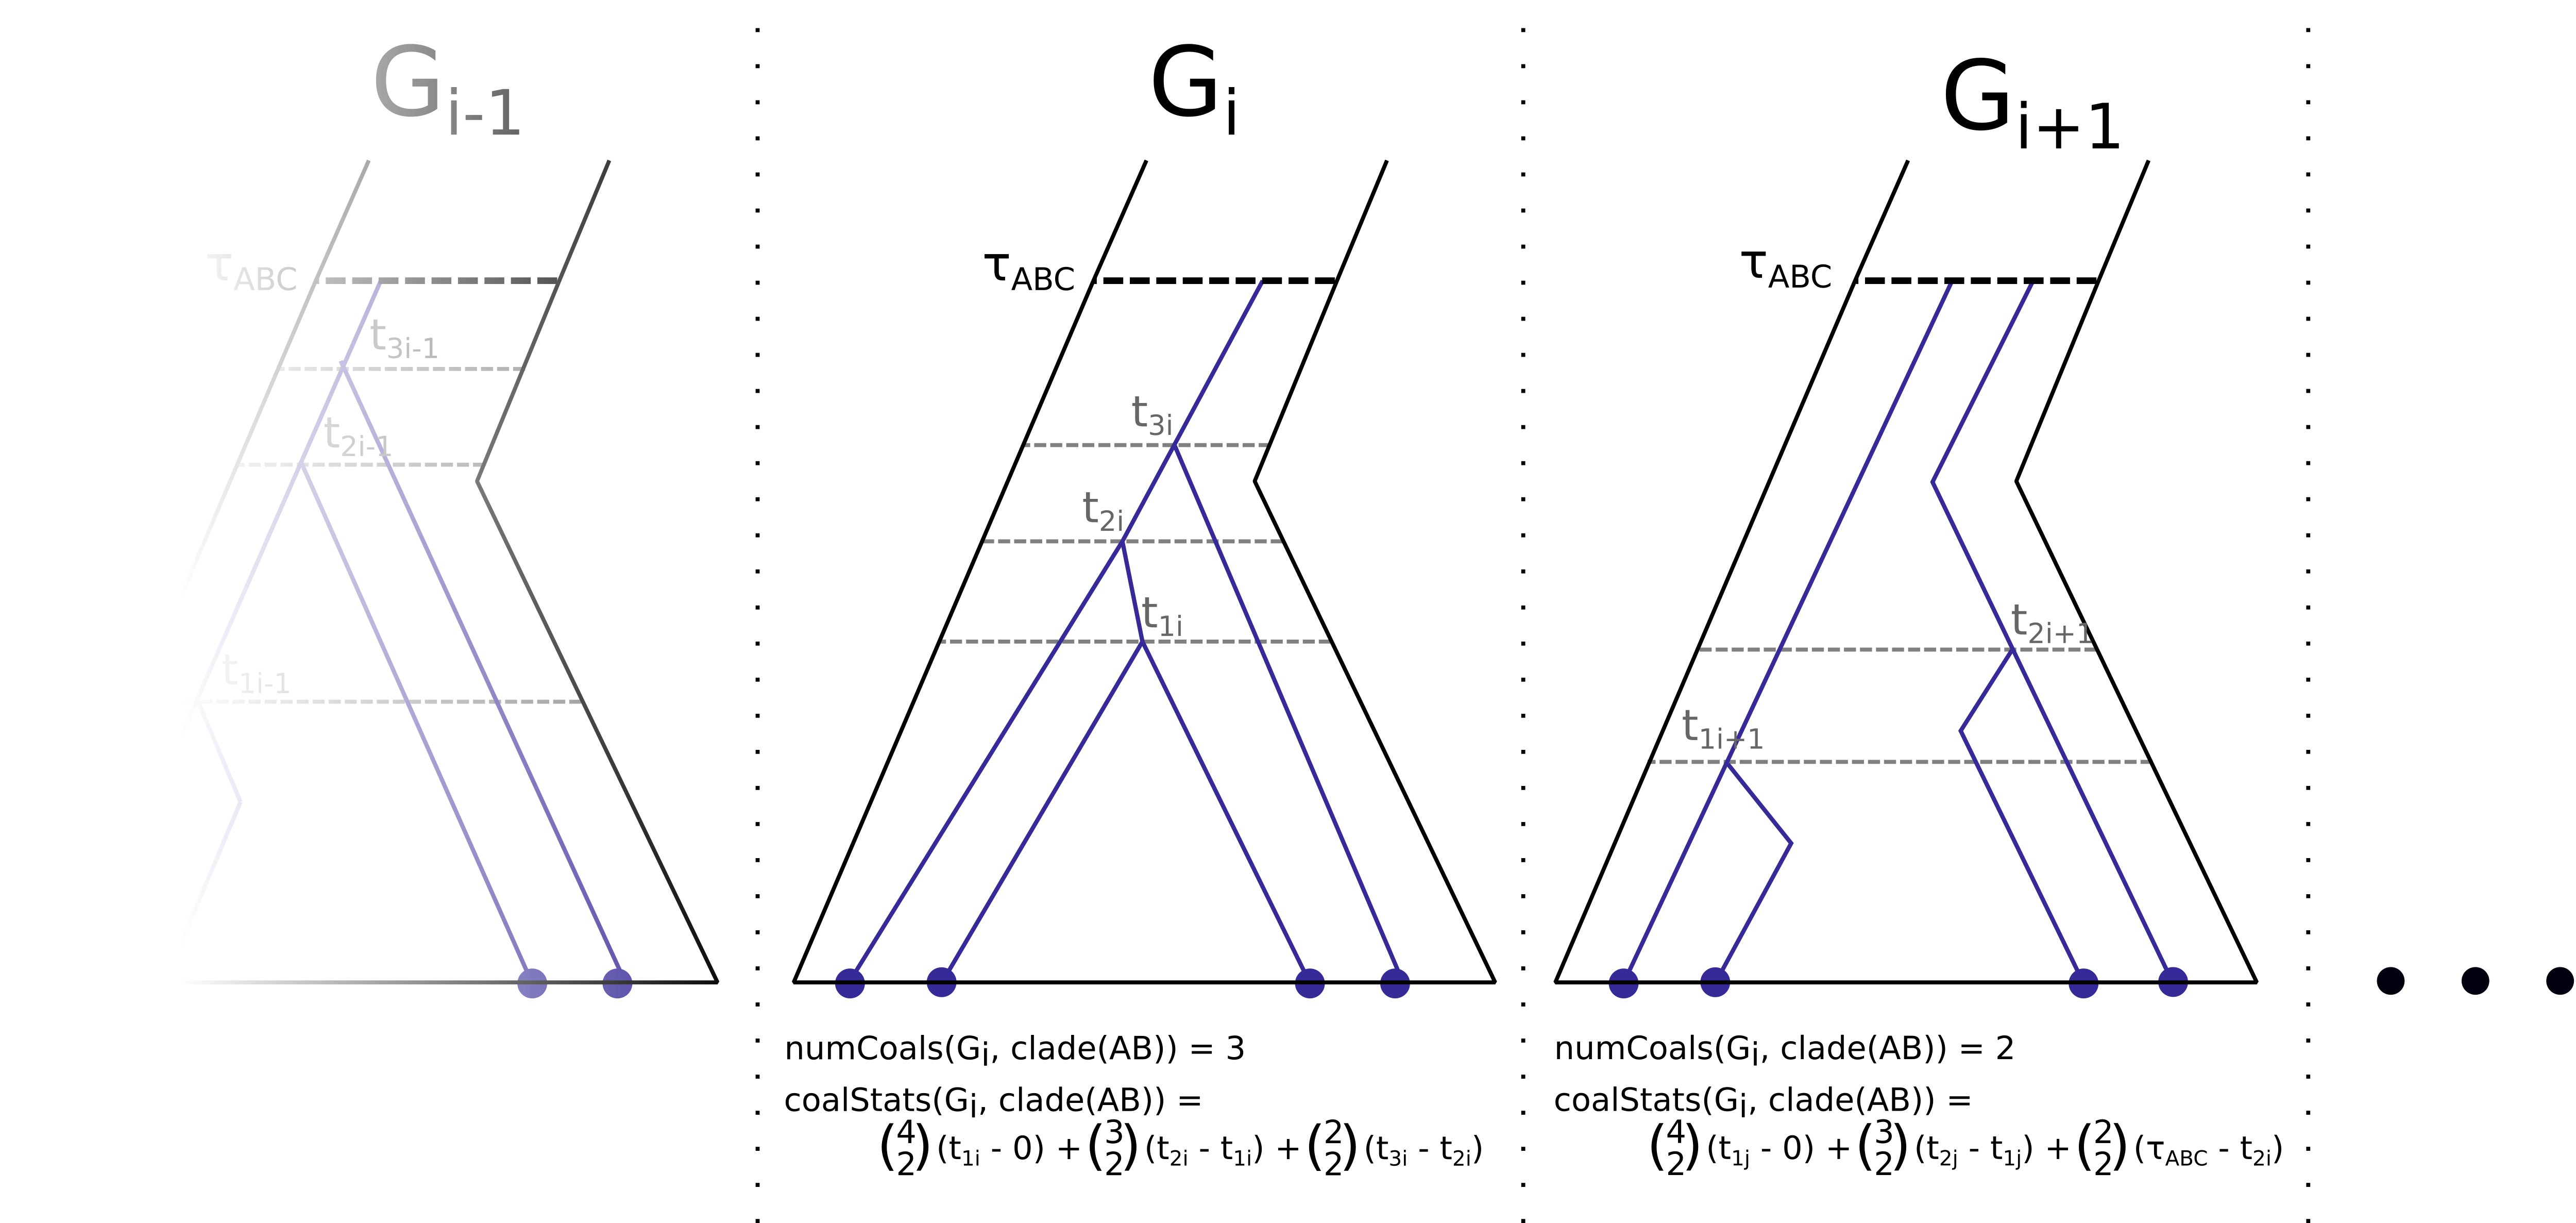
\includegraphics[width=1.0\textwidth]
{multiple_loci}
\captionsetup{width=.8\textwidth}
\caption{The sufficient statistics, \textit{numCoals} \& \textit{coalStats}, are calculated per clade using the time intervals $\Ip$, and are accumulated across loci.\\
%
ALTERNATIVE: The contribution of $clade(AB)$ to $\ln \left( P(\G| \T,\Mref) \right)$ is the sum of it's contributions to the genealogy log-likelihood of all loci. These are calculated for loci $l_i$, using the set of intervals $\mathcal{I}(clade(AB),l_i)$.\\
%
ALTERNATIVE: The sufficient statistic $coalStat(G, clade(AB))$ is calculated by accumulating the Kingman Coalescent genealogy log-likelihod across loci. The contribution of each loci is calculated via the set of intervals $\mathcal{I}(clade(AB),l_i)$. The sufficient statistic $numCoals(G, clade(AB))$ is simply the sum across loci of the amount of coalescnece events inside $clade(AB)$.\\
%
\textcolor{red}{TODO - fix subscript in right genealogy. Also fix fading line above and below left genealogy. Also add another fading genealogy to the right, instead of the dot-dot-dot. Also maybe write somewhere the this is $clade(AB)$}}
\label{fig:multiple_loci}
\end{figure}


The summary statistics $\{~numCoals(\G,p),~~ coalStats(\G,p)~\}_p$~ and ~$\{~numMigs(\G,b),~~ migStats(\G,b)~\}_b$ satisfy our first objective in that their number depends on the complexity of the reference model $\Mref$ but not on the size of the data.
%
They also partly satisfy the second condition, because statistics computed for a given set of local genealogies and given values of divergence times enable computation of the likelihood $P(\G|\T,\Mref)$ for any set of values of the population size and migration rate parameters.
%



\subsection{Recursive Calculation of Sufficient Statistics for Multiple Clade Reference Models}
To support all valid reference models generated by the reference construction process (subsection \ref{Constructing a Reference Model}) we must calculate all summary statistics for every population in every valid reference model.
%
Fortunately, we note that any part of the topology of $\Mref$ which was not transformed during the reference model creation process has the exact same statistics in the $\M$ and in $\Mref$. This allows us to reuse statistics already gathered by \gp for many populations of the reference model. What remain to be calculated are sufficient statistics for all possible clades-  \[\{~numCoals(\G,clade(p)),~~ coalStats(\G,clade(p))~\}_{p\in P_{ref}}\]

To achieve this in an efficient manner, calculation of $numCoals$ and $coalStats$ is done recursively down the population phylogeny of $M$ (see pseudo-python code below). This is done using a function for computing $coalStats$ given a sorted list of intervals (\pythoninline{calculate_coal_stats}), as well as accessors to data from \gp (\pythoninline{num_coals_from_gphocs} \& \pythoninline{sorted_intervals_from_gphocs}):
%

\begin{python}


def recursive_num_coals(pop):
    """recursively calculate and store num of coalescence
    events in clade(pop) as well as all descendant clades"""

    pop_num_coals = num_coals_from_gphocs(pop)

    if is_leaf(pop):
        return pop_num_coals

    left_num_coals = recursive_num_coals(pop.left)
    right_num_coals = recursive_num_coals(pop.right)

    current_num_coals = pop_num_coals + left_num_coals + right_num_coals
    store(current_num_coals)

    return current_num_coals


def recursive_coal_stats(pop):
    """recursively calculate and store coalescence stats
    of clade(pop) as well as all descendant clades"""

    pop_intervals = sorted_intervals_from_gphocs(pop)

    if is_leaf(pop):
        return pop_intervals

    left_intervals = recursive_coal_stats(pop.left)
    right_intervals = recursive_coal_stats(pop.right)
    merged_intervals = merge_sort(left_intervals, right_intervals)

    clade_intervals = merged_intervals.append(pop_intervals)

    clade_coal_stats = calculate_coal_stats(clade_intervals)
    store(clade_coal_stats)

    return clade_intervals

\end{python}

\subsection{Calculating Comb Reference Model Genealogy Likelihood}

Formula \ref{eq:gen_ratio_comb} shows how for a reference model created by comb-collapsing the root population, contribution of the genealogy-likelihood to the model-pairing conditional is reduced to contribution of the portion of genealogies above $\tmin$ - 
\[\frac{ P({\G}_{c|>\tmin}|\M_0,\theta_0=\troot) }{ P(\G_{>\tmin}|\M,\T)} ~ .\]

When comb-collapse is applied to a subtree, we apply the same idea to the portion of the genealogy contained in that subtree. Figure 3 Illustrates the intervals relevant for genealogy-likelihood calculation in the hypothesis and reference models. 


As in the case for clade reference models, we wish to calculate statistics for all viable comb reference models after only one MCMC chain. We do this by storing for every ancestral population $p$ the log of the denominator $~ln(P(\G_{>\tmin}|\M,\T))~$ and the two sufficient statistics involved in the calculation of the enumerator - ($\{~numCoals(\G,comb(p)),~~ coalStats(\G,comb(p))~\}_p$). 
%
This is again calculated recursively down the population phylogeny of $\M$, but the function \pythoninline{calculate_coal_stats} now takes into account only intervals inside the subtree of $p$ and above $\tmin$.


\begin{figure}[h]
\centering
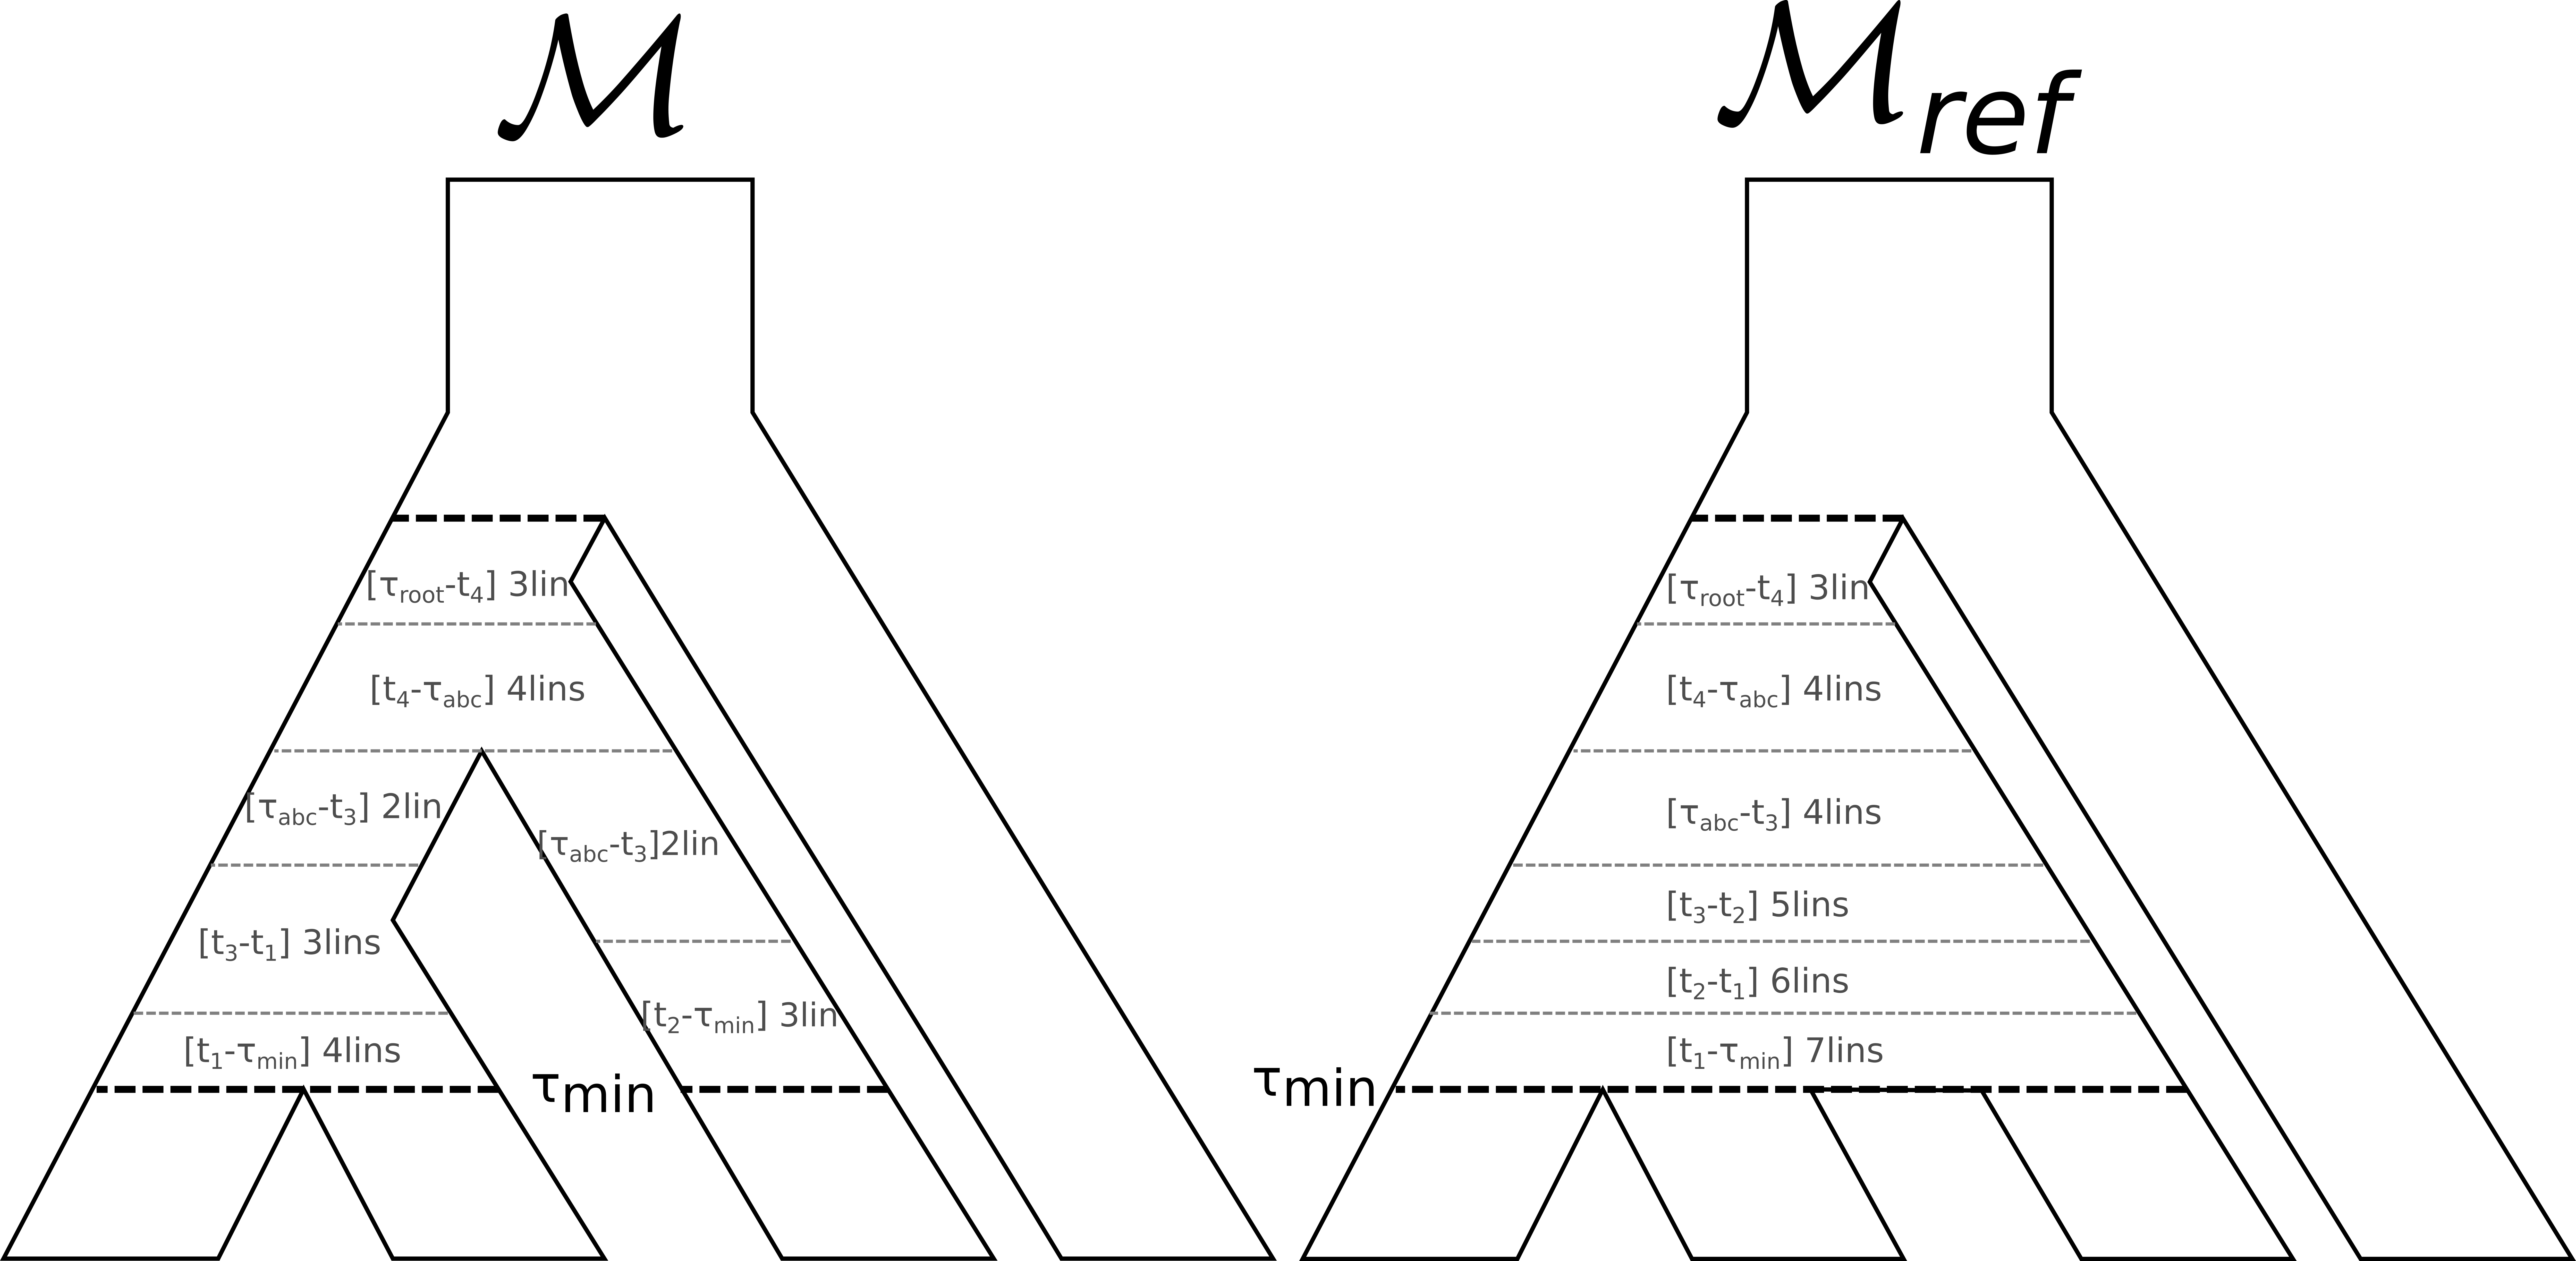
\includegraphics[width=1.0\textwidth]
{hyp_and_comb_intervals}
\captionsetup{width=.8\textwidth}
\caption{In comb reference models, genealogy-likelihood need only be calculated strictly within the bounds of the comb population $comb(p)$. Outside this area of the topology, genealogy-likelihood of the reference and hypothesis models cancels out in the Model-Pairing Conditional. \textcolor{red}{TODO - color the model branches}}
\label{fig:calculate_hyp_stats_above_tmin}
\end{figure}

\newpage
\section{Technicalities and Code}


\subsection{Debugging results}

When examining results of \gp calculations for mcref we were faced with the challenge of validating our results. \#explanation-on-why-this-was-needed. We wished to double-check every statistic emitted, with the simple goal of predictably and reliably reaching our intended calculation.

This was accomplished using a variaty of techniques, restricted by the target statistic and reference model and by the tools at our disposal. 


\begin{itemize}

\item \underline{in comb: compare leaves when comb-age:=inf. Compare root comb when comb-age:=0}

To validate our comb coal-stats calculations we permanantly set the comb-age to various values, allowing us to predict results. When setting a high comb-age (essentially infinite), we asserted That the coal-stats of comb-leaves is equal to the leaf population stats calculated by \gp. When setting comb-age to zero (thus reducing the comb to a clade), we asserted that the coal-stats of the root-comb is equal those of the null reference model (calculated independently by the clade algorithm and by a preexisting \gp implementation).



\item \underline{in clade: compare "leaf clade" with leaf. Compare root-clade with \gp -calculated root-clade}
To assert clade coal-stats, we applied techniques similiar to those used for the comb algorithm. Leaf-rooted clades were compared with leaf stat calculated by \gp and the root-clade (aka the null reference modle) was compared with independantly calculated stats for the null reference model. 

\item \underline{In tau bounds: monotonouty up pop tree. Assert diff(bound, tau) neg correlated with \#loci}

We expected each tau bound to decrease towards its corresponding population tau as the number of loci increases. This due to an increase in the number of coalescence events, leading to an increase in chance of some coalescence event occurring closer to the population tau. We ran a simple set of \gp experiments using the same sequence data, changing only the number of loci in-use. We observed a negative correlation between the number of loci and the tau bound, as expected.

Another simple validation we performed was asserting that bounds are monotonously decreasing down the population tree.

\end{itemize}

\subsection{McRef Code}

\begin{itemize}
\item \underline{configuration}

When setting up mcref, several parameters are configured. The parameters pertain to standard I/O (e.g. where the trace data files are stored and where to store output), to the phylogenic population models (i.e. the structure of the reference and hypothesis models), to \gp configuration (e.g. what alpha \& beta to use for gamma priora, what print multipliers were applied to trace data when emitted by gphocs etc.), to statistical calculations (e.g. how many bootstrap iterations to run during confidence calculation and how much burn-in and sample-skip to use in genealogy likelihood calculation) and to debugging (e.g. what debug calculations to run and visualizations to emit). 

\item \underline{calculating kingman coalescence and kingman migration for the reference model}

Calculating the reference model genealogy likelihood was done using the standard kingman coalescence model, in the same manner implemented in gphocs. The theta of the actual comb/clade population was set to that of the population at the top of the comb/clade and plugged into \#gen\_ld\_ln-formula. 

\item \underline{calculating tau priors for hypothesis and reference models}
tau priors for the hypothesis model were calculated using the same gamma-distribution used by gphocs, based on taus emitted during the \gp run. tau priors for the reference model were calculated using a uniform distribution based on tau-bounds, as described in the chapter about tau bounds.

\item \underline{estimating variance using bootstrap}

In an attempt to estimate the variability of the genealogy likelihood calculation, bootstrap estimations of the rbf were repeatedly sampled from the trace data. 


\item \underline{optimizing runtime (lazily caching trace files, multiprocess concurrently running comparisons, )}

With the goal of optimizing the practical run-time and usability of mcref, several techniques were employed; trace data files, which are repeatedly read and used, are lazily loaded and cached in each mcref process. Multiple mcref experiments are launched using a single command and are cocurrently run in multiple processes, eventually aggregating summary results to a single log file. 

\item \underline{visualizing results}

To clarify results and to help in the understanding and debugging of mcref runs, several visual outputs were developed. each mcref run emits plots of the genealogy-log-likelihood of the reference model and of the hypothesis model, as well as a plot of the rbf calculation across \gp iterations and a plot of the harmonic mean of likelihood of the hypothesis model.

\item \underline{debugging visualizations}

Multiple debug plots are also emitted by mcref. Their goal is to help the researcher assert the experiment was executed as planned. These plots contain the kingman coalescence and kingman migration of every population and migration in both the hypothesis and reference models. They also contain the aggregate coal-stats of the hypothesis and reference model, allowing us to assert that coal-stats of a reference model always exceed those of it's hypothesis \#here-goes-an-explanation-of-the-previous-sentence. 
\end{itemize}



\section{Results}
Results-go-here

\section{Discussion}

\newpage

\section{References}
Bibliography-goes-here


\newpage


\appendix
\newcommand{\anc}{\geq_\Tr}
\newcommand{\nanc}{\ngeq_\Tr}
\section{\texorpdfstring{The conditional distribution $\Pref(\taus|\G)$ for models without migration}{Conditional distribution without migration}}\label{ap:cond_nomig}

Recall that the model-pairing conditional distribution for the null model $\M_0$ with a model $\M$ with no migration bands is determined by specifying a conditional
distribution for the divergence times given the genealogy, $\Pref(\taus|\G)$ (Equation \ref{eq:rbf_null}).
%
To guarantee the model-pairing condition of Equation \ref{eq:pref_support} we need to ensure that  $\Pref(\taus|\G)=0$ whenever $P(\G|\taus,\M)=0$.
%
This is done by determining when a given collection of genealogies is \emph{embeddable} in a population phylogeny.
%
Consider a population phylogeny $\Tr$ with given divergence times $\taus=\taus$ and a collection of local genealogies $\G$ whose leaves are mapped to
leaves of $\Tr$.
%
Each vertex $v$ in a local genealogy corresponds to a coalescent event at time $t(v)$, and each vertex $p$ in the population phylogeny corresponds to a population
whose life span is between $\tau(p)$ and $\tau(parent(p))$. (if $p$ is a leaf population then $\tau(p)=0$ and if $p$ is the root population then $\tau(parent(p))=\infty$.)
%
A valid embedding is defined as follows:
%
\begin{definition}\label{def:embed}
 An embedding of a collection of local genealogies $\G$ in a timed population phylogeny $(\Tr,\taus)$ is a mapping, $pop:\G\rightarrow\Tr$,
 which satisfies the following conditions for every coalescent event $v$ in $\G$:
 \begin{enumerate}
  \item $pop(v)$ is alive at time $t(v)$:~~ $\tau(pop(v)) ~<~ t(v) ~\leq~ \tau(parent(pop(v)))$~.\label{cond:time}
  \item $pop(parent(v))$ is ancestral (or equal) to $pop(v)$:~~ $pop(parent(v)) \anc pop(v)$.\label{cond:anc}
 \end{enumerate}
\end{definition}

Note that condition \ref{cond:anc} can be extended to show that for every $u$ ancestral to $v$, we have $pop(u) \anc pop(v)$.
%
Another interesting observation about embeddings is that they are \textbf{unique given the population assignments to the leaves in} $\G$.
%
To prove this, consider an arbitrary coalescent event $v$ in $\G$, and let $l$ be some some leaf in the subtree rooted at $v$ (we denote this set by $leaves(v)$).
%
Condition \ref{cond:anc} implies that $pop(v) \anc pop(l)$, and there is exactly one population ancestral to $pop(l)$ that also satisfies condition \ref{cond:time} (i.e. alive at time $t(v)$).
%
This argument can also be used to establish a sufficient and necessary condition for the existence of an embedding.
%
\begin{definition}[$mrcaPop$]\label{def:tmrca_pop}
 Given a coalescent event $v$ in a local genealogy whose leaves are assigned to the leaves of a population phylogeny $\Tr$,
 let ${mrcaPop(v)}$ denote the most recent population ancestral to all populations in $\{pop(l):l\in leaves(v)\}$.
\end{definition}

\begin{lemma}\label{lem:embed}
 A collection of local genealogies $\G$ has an embedding in a timed population phylogeny $(\Tr,\taus)$ iff every coalescent event $v$ in $\G$ satisfies $t(v) > \tau(mrcaPop(v))$.
\end{lemma}
\begin{proof}
 ~\\
 $\Rightarrow$:~~ Consider an embedding $pop:\G\rightarrow\Tr$, and let $v$ be an arbitrary coalescent event in $\G$.
 Condition \ref{cond:anc} implies that $pop(v)\anc pop(l)$ for all $l\in leaves(v)$, and thus $pop(v)\anc mrcaPop(v)$.
 By condition \ref{cond:time}, we get $t(v) > \tau(pop(v)) \geq \tau(mrcaPop(v))$.\\
 $\Leftarrow$:~~ Let $v$ be an arbitrary coalescent event in $\G$, and assume that $t(v) > \tau(mrcaPop(v))$. This means that there is a (unique) population, $p^*$,
 ancestral to $mrcaPop(v)$ that is also alive at time $t(v)$ (i.e., $\tau(p^*) ~<~ t(v)$\\
 $\leq~ \tau(parent(p^*))$). Define the embedding $pop$ by mapping $v$ to population $p^*$.
 Condition \ref{cond:time} is guaranteed by construction. 
 Condition \ref{cond:anc} is proved by considering an arbitrary coalescent event $v$ and its parent $u=parent(v)$.
 By construction we get that $pop(u),pop(v) \anc mrcaPop(v)$ (because $mrcaPop(u)\anc mrcaPop(v)$).
 Thus either $pop(v)\anc pop(u)$ or $pop(u)\anc pop(v)$.
 Condition 1  implies that $pop(v)$ cannot be strictly ancestral to $pop(u)$ via the following sequence of inequalities:
 %
 $$\tau(parent(pop(u)) ~\geq~ t(u) ~\geq~ t(v) ~>~ \tau(pop(v))~.$$
 %
 Hence, $pop(u)\anc pop(v)$, establishing condition \ref{cond:anc}.
\end{proof}

Lemma \ref{lem:embed} can be used to establish the feasible range of every divergence time $\tau_p$ by noting that a given divergence time
is feasible (i.e., $P(\G|\tau_p=\tau,\M)>0$) if and only if the values of the other divergence times can be set to allow the embedding of $\G$ in $(\Tr,\taus)$.

\begin{corollary}\label{cor:tau_bound}
 Let $\G$ be a  collection of local genealogies whose leaves are mapped to leaves of a population phylogeny $\Tr$. Then for every population $p$ in $\Tr$, we have:
 %
 $$P(\G|\tau_p=\tau,\M)>0 \textbf{~~iff~~}  0\leq \tau < \min \{t(v):mrcaPop(v)\anc p\} ~.$$
\end{corollary}

Given $\G$, we may compute $divBound(p|G) \eqdef \min \{t(v):mrcaPop(v)\anc p\}$ for every population $p$ in $\Tr$, and then define $\Pref(\taus|\G)$ as a uniform distribution over the
multi-dimensional rectangle defined by $\tau_p \in [0,divBound(p|G))$.

\textbf{TBA: explicit description of procedure for computing $divBound(p|G)$.}

\section{\texorpdfstring{The conditional distribution  $\Pref(\taus,\Gm|\Gc)$ for models with migration}{Conditional distribution with migration}}\label{ap:cond_mig}

-- TBA --



\end{document}
